
\chapter{Type Inference}
\vspace{-1em}
\begin{center}
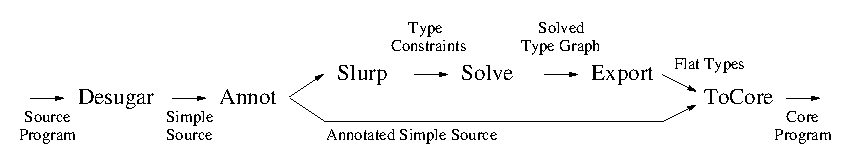
\includegraphics{3-Inference/fig/intro/overview}
\end{center}

The above diagram gives an overview of our compilation process. The source program is first desugared into a simpler language, and then annotated with type variables that serve as ``hooks'' for type constraints. Type constraints relating these hook variables are extracted (slurped) from the annotated program. The constraints are solved, which produces a solution in the form of a type graph. The solution is a graph because it can contain cycles through effect and closure information due to the definitions of recursive functions. This was discussed in \S\ref{System:Effects:recursive}. We then extract flat, non-graphical types for each of the hook variables, and use this information to translate the annotated source program into the core language.

This chapter concerns the annotation, constraint slurping, solving and export stages. We give the motivation for our overall approach in \S\ref{Inference:BindingOrder}, and discuss the use of type graphs. We define the simplified source language in \S\ref{Inference:Language}, and go on to discuss the annotation process and constraint slurping. Constraint solving is outlined in \S\ref{Inference:Reduction} and \S\ref{inference:generalisation}, where \S\ref{Inference:Reduction} deals with the reduction of monomorphic constraints, and \S\ref{inference:generalisation} discusses type generalisation and the extraction of flat types. In practice we also keep track of how type schemes are instantiated. This information is used when translating the source program to core, but we do not discuss this or other details of the translation in this thesis.

Section \S\ref{Inference:Projections} extends the source language and inference algorithm with support for type directed projections, and \S\ref{inference:ordering} discusses how to handle mutual recursion in the presence of such projections. Section \S\ref{inference:type-classes} discusses the built-in type class constraints such as $\iPure$ and $\iShape$, and \S\ref{inference:errors} considers how to produce reasonable error messages.





\clearpage{}

\section{Binding order and constraint based inference}
\label{Inference:BindingOrder}

When performing type inference for Haskell, a binding dependency graph is used to determine which groups of bindings are mutually recursive. This graph is also used to sort the binding groups so that their types are generalised before they need to be instantiated~\cite{jones:typing-haskell}. Unfortunately, due to the inclusion of type directed projections, a similar dependency graph cannot be extracted from Disciple programs before type inference proper. 

Consider the following program:

\qq\qq
\begin{tabular}{ll}
	$\ifunOne \ x$		& $= 1 + \ifunTwo x \ 5$	\\
  	$\ifunTwo \ x \ y$	& $= x + y$
\end{tabular}
\bigskip

As the body of $\ifunOne$ references $\ifunTwo$, we should generalise the type of $\ifunTwo$ before inferring the type of $\ifunOne$. It is easy to extract such dependencies from Haskell programs because at each level of scope, all bindings must have unique names. However, in Disciple programs, projections associated with different type constructors can share the same name. For example:

\qq\qq
\begin{tabular}{ll}
	\mc{2}{$\kproject \ \iTone \ \kwhere$} \\
	& $\ifieldOne \ x \ =  (x, \ 5)$ \\
\\
	\mc{2}{$\kproject \ \iTtwo \ \kwhere$} \\
	& $\ifieldOne \ x \ =  (x, \ ``\texttt{hello}")$
\end{tabular}
\bigskip

We have defined two projections named $\ifieldOne$, one for constructor $\iTone$ and one for constructor $\iTtwo$. Now consider what happens when we perform a $\ifieldOne$ projection in the program:

\qq\qq
\begin{tabular}{ll}
	$\ifun \ x  = \dots  \ x \odot \ifieldOne \ \dots$
\end{tabular}
\bigskip

This $x \odot \ifieldOne$ projection will be implemented by one of the instance functions above, but we cannot determine which until we know the type of $x$. For Disciple programs, there is no easy way to determine the binding dependency graph, or to arrange the bindings into an appropriate order before inferring their types. Instead, we must determine how the bindings depend on each other on the fly, during inference.

This implies that our inference algorithm cannot be entirely syntax directed. When inferring the type of $\ifun$, once we determine which instance function to use for the $\odot \ifieldOne$ projection, we may discover that this type hasn't been inferred yet either. We must then stop what we're doing and work out the type of the instance function, before returning to complete the type of $\ifun$. In general, this process is recursive. Work on the types of several bindings may need to be deferred so that we can first determine the type of another. 

We manage this problem with a constraint based approach, similar to that used by Heeren in the Helium compiler~\cite{heeren:generalising-hm, heeren:constraint-type-inferencing, heeren:top-quality-error-messages}. We extract type constraints from the desugared source program, solve them, and then use the solution to translate the desugared code into the core language, while adding type annotations. By approaching type inference as the solution of a set of constraints instead of a bottom-up traversal of the program's abstract syntax tree, we make it easier to dynamically reorder work as the need arises. This framework also helps to manage our extra region, effect and closure information. Once we have a system for expressing and solving general type constraints, the fact that we have constraints of different kinds does not add much complexity to the system. Constraint based systems also naturally support the graphical effect and closure terms discussed in \S\ref{System:Effects:recursive}, as well as providing a convenient way to manage the information used to generate type error messages.

Our system has some similarity to the one use by $\textrm{ML}^\textrm{F}$~\cite{remy:graphic-type-constraints}, though we do not consider higher rank types. We believe our system could be extended to support them, but we have been mainly interested in the region, effect and closure information, and have not investigated it further. We also derive inspiration from Erwig's visual type inference~\cite{erwig:visual-type-inference}, and the graphs used by Duggan~\cite{duggan:explaining-type-inference} to track the source of type errors. However, unlike their work we do not draw our type graphs pictorially. We have found that the addition of region, effect and closure information, along with the associated type class constraints, tends to make these two dimensional diagrams into ``birds nests'' with many crossing edges, which hinders the presentation. Instead, we simply write down the constraints as equations, and try to imagine the graph being separated into several two dimensional layers, one for each kind. Such graphs might make an interesting target for work on computer aided visualisation as we know of no tool to generate a suitably pleasing diagram.



%!TEX root = ../Main.tex

\begin{figure}
\boxfig{
\begin{tabbing}
MMM              \= MM   \= MMMMMMMMMMMMMMMMM   \= MMM \= MM \= MMMMMMMM    \kill
\textbf{Indices} \> \>                 \> \textbf{Names} \\
$ix$ \> $\to$   \> (debruijn index)    \> $a,~ r,~ e$ \> $\to$ \> (type variables)     \\
$p$  \> $\to$   \> (region identifier) \> $z$         \> $\to$ \> (term variables)     \\
$l$  \> $\to$   \> (store location)
\\
\\

\textbf{Kinds} ($k$)\\
$\mkind$
        \> ::=   \> $\kcData ~~|~~ \kcRegion ~~|~~ \kcEffect$
        \> (kind constructors)
\\
        \> $~|~$ \> $\mkind \kto \mkind$ 
        \> (function kind)
\\
\\


\textbf{Types} ($t,~ r,~ e$)\\
$\mtype$  
        \> ::=  \> $ix\bra{a}$
        \> (debruijn index\bra{variable})
\\
        \> $~|~$  \> $\forall \bra{a} : \mkind.~~ \mtype$
                        $~|~$ $\mtype~~ \mtype$
        \> (universal quantifier, type application)
\\
        \> $~|~$  \> $\mtype ~+~ \mtype$
                        $~|~$ $\bot$           
        \> (effect join and bottom) 
\\        
        \> $~|~$  \> $\mtycon_n$        
        \> (type constructor)
\\      
        \> $~|$   \> $\trgn{p}$
        \> (region handle)
\\
\\


\textbf{Type Constructors} ($\mtc$)\\
$\mtycon_0$ 
        \> ::=  \> $(\to)
                        ~~|~~ \tcUnit
                        ~~|~~ \tcBool
                        ~~|~~ \tcNat$
\\
$\mtycon_1$ 
        \> ::=  \> $\tcRead
                        ~~|~~ \tcWrite
                        ~~|~~ \tcAlloc$
\\
$\mtycon_2$ 
        \> ::=  \> $\tcRef$
\\ 
\\


\textbf{Values} ($v$)\\
$\mval$ \> ::=  \> $ix\bra{z} ~~|~~ \mconst$ 
        \> (debruijn index\bra{variable}, constant)
\\
        \> $~|$ \> $ \lambda \bra{z} : \mtype.~ \mexp
               ~~|~~ \Lambda \bra{a} : \mkind.~ \mexp$
        \> (value and type abstraction)
\\
        \> $~|$ \> $\vloc{l}$
        \> (store location)
\\
\\


\textbf{Expressions} ($x$)\\
$\mexp$ \> ::=  \> $\mval
                        ~~|~~ \mval~~ \mval
                        ~~|~~ \mval~~ \mtype$
        \> (value, value and type application)
\\
        \> $~|$ \> $\xlet{\bra{z}}{\mtype}{\mexp}{\mexp}$
        \> (let-binding)
\\
        \> $~|$ \> $\mop_n~ \ov{\mval}^{\; n}$
        \> (fully applied pure operator)
\\
        \> $~|$ \> $\xprivate{\bra{r}}{\mexp}$
        \> (define a private region)
\\
        \> $~|$ \> $\xextend{\mtype}{\bra{r}}{\mexp}$
        \> (extend an existing region)
\\
        \> $~|$ \> $\kalloc~~ \mtype~~ \mval$
        \> (allocate a store binding)
\\
        \> $~|$ \> $\kread~~~~  \mtype~~ \mval$
        \> (read a store binding)
\\
        \> $~|$ \> $\kwrite~~ \mtype~~ \mval~~ \mval$
        \> (write a store binding)
\\
\\


\textbf{Constants} ($c$)\\
$const$ \> ::=  
        \> $\tt{unit} 
                ~|~ \tt{tt}
                ~|~ \tt{ff}
                ~|~ \tt{0} 
                ~|~ \tt{1} 
                ~|~ \tt{2}
                ~|~ ...$
        \> (data constants)
\\
\\

\textbf{Pure Operators} ($o$)\\
$\mop_1$
        \> ::=  \> $\tt{isZero} 
                        ~~|~~ \tt{succ}$
        \> (pure operators)
\end{tabbing}
} % boxfig
\medskip
\caption{\SystemFre grammar.}
\label{f:Language}
\end{figure}


 
\clearpage{}
\subsection{Example: type constraints}

The following contraint tree is for our $\imap$ example:

\begin{tabbing}
MMMM 	\= MM \= MM \= MM \= MM \= MM \= MM \= MM \= MM \= MM \= MM \= MM \= MM \kill

GROUP $\{ \imap \}$ \\	
	\> $s_0$	\> $ = s_{19}$ \\
	\> $e_0$	\> $\tme e_1 \lor e_{19}$
\\[1ex]
	\> LET \ $\imap$ \\
	\> 		\> $s_{map}$	\> $ = s_1$ 
\\[1ex]
	\>		\> LAMBDA \ \{$f$\} \\
	\>		\> 		\> $s_1$	\> $ = s_f    \lfuna{e_2 \ c_1} s_2$ \\
	\>		\>		\> $c_1$ 	\> $\tme \imap : s_{\imap}$ 
\\[1ex]
	\>		\> 		\> LAMBDA \ \{$xx$\} \\
	\>		\>		\> \> $s_2$		\> $ = s_{xx} \lfuna{e_3 \ c_2} s_3$ 
	\>		\>		\> \> $c_2$		\> $\tme \imap : s_{\imap} \lor \ f : s_f$ 
\\[1ex]
	\>		\>		\> \> $s_3$		\> $ = s_6$ 
	\>		\>		\> \> $e_3$ 		\> $\tme \iReadH s_4 \lor e_6 \lor e_7$  \\
	\>		\>		\> \> $s_3$		\> $ = s_8$  \\	
	\>		\>		\> \> $s_4$		\> $ = s_5$  \\
	\>		\>		\> \> $s_4$		\> $ = s_7$  \\
	\>		\>		\> \> $s_5$		\> $ = \iList \ r_5 \ a_5$ \\
	\>		\>		\> \> $s_7$		\> $ = \iList \ r_7 \ a_7$ \\
	\>		\>		\> \> $s_x$		\> $ = a_7$ \\
	\>		\>		\> \> $s_{xs}$		\> $ = \iList \ r_7 \ a_7$ \\
	\>		\>		\> \> $s_4$		\> $ = \rINST \ s_{xx}$  \\
	\>		\>		\> \> LAMBDA \ $\emptyset$	\\
	\>		\>		\> \> \> $s_6$		\> $ = \rINST \ s_{\iNil}$ 
\\[1ex]
	\>		\>		\> \> LAMBDA \ $\{ x, \ xs \}$					\\
	\>		\>		\> \> \> $s_9$		\> $ = s_{14} \lfuna{e_{8a} \ c_8} s_8$ 
	\> 		\> 		\> \> \> $e_8$		\> $\tme e_9 \lor e_{14} \lor e_{8a}$ 
\\
	\>		\>		\> \> \> $s_{10}$	\> $ = s_{11} \lfuna{e_{9a} \ c_9} s_9$ 
	\>		\>		\> \> \> $e_9$		\> $\tme e_{10} \lor e_{11} \lor e_{9a}$ 
\\[1ex]
	\>		\>		\> \> \> $s_{10}$	\> $= \rINST \ s_{\iCons}$  
\\[1ex]
	\>		\>		\> \> \> $s_{12}$ 	\> $= s_{13} \lfuna{e_{11a} \ c_{11}} s_{11}$ 
	\>		\>		\> \> \> $e_{11}$ 	\> $\tme e_{12} \lor e_{13} \lor e_{11a}$  
\\[1ex]
	\>		\>		\> \> \> $s_{12}$	\> $= \rINST \ s_f$ \\
	\>		\>		\> \> \> $s_{13}$	\> $= \rINST \ s_x$ \\
	\>		\>		\> \> \> $s_{15}$	\> $= s_{18} \lfuna{e_{14a} \ c_{14}} s_{14}$ 
	\>		\>		\> \> \> $e_{14}$	\> $\tme e_{15} \lor e_{18} \lor e_{14a}$ 
\\[1ex]
	\>		\>		\> \> \> $s_{16}$	\> $= s_{17} \lfuna{e_{15a} \ c_{15}} s_{15}$ 
	\>		\>		\> \> \> $e_{15}$	\> $\tme e_{16} \lor e_{17} \lor e_{15a}$ 
\\[1ex]
	\>		\>		\> \> \> $s_{16}$	\> $= \rINST \ s_{map}$ \\
	\>		\>		\> \> \> $s_{17}$	\> $= \rINST \ s_{f}$ \\
	\>		\>		\> \> \> $s_{18}$	\> $= \rINST \ s_{xs}$
\\[1ex]
	\> $s_{20}$	\> $= s_{23} \lfuna{e_{19a} \ c_{19}} s_{19}$ \> \> \>
	\> $e_{19}$	\> $= e_{20} \lor e_{23} \lor e_{19a}$ 
\\[1ex]
	\> $s_{21}$	\> $= s_{22} \lfuna{e_{20a} \ c_{20}} s_{20}$ \> \> \>
	\> $e_{20}$	\> $= e_{21} \lor e_{22} \lor e_{20a}$
\\[1ex]
	\> $s_{21}$	\> $= \trm{INST} \ s_{\imap}$ \\
	\> $s_{22}$	\> $= \trm{INST} \ s_{\idouble}$ \\
	\> $s_{23}$	\> $= \trm{INST} \ s_{\ifoo}$ 
\end{tabbing}

\clearpage{}

The constraint tree echos the abstract syntax tree. We have retained the overall structure of the program, while dispensing with details such as distinction between case alternatives and lambda abstractions, and the order of function applications. Once constraints have been extracted, the inference algorithm can ignore the source program entirely. In our real implementation we use a source language that has more sugar than the one presented here, but the constraint language is the same.

Before discussing how to actually solve the constraints, note that there are several degrees of freedom in their ordering. Within a particular LAMBDA, LET or GROUP block it is always safe to move $=$ or $\tme$ constraints earlier in the block. It is also safe to move these constraints up and earlier in the tree, such as moving $s_{\imap} = s_1$ so it appears directly after $e_0 \tme e_1 \lor e_{19}$. Moving these constraints higher up in the tree means they will be considered earlier, and such modifications will not degrade the final constraint solution. It is also safe to change the order of LAMBDA or LET blocks at the same level. This simply corresponds to changing the order of let-bindings or case-alternatives in the original program. On the other hand, in general it is \emph{not} safe to move INST constraints as they control the order in which types are instantiated.

Although we will discuss recursion more fully in \S\ref{inference:ordering}, the structure of the constraints reveals that $\imap$ is recursively defined. This is evident from the fact that $s_{16} = \trm{INST} \ s_{\imap}$, present in the lower quarter of the list, appears inside the LET $\imap$ block. This constraint corresponds to a recursive use of $\imap$. This is in contrast to $s_{21} = \rINST \ s_{\imap}$ which appears outside the block and corresponds to a non-recursive use. Without polymorphic recursion, all recursive uses of let-bound variables should be at identical types, so we will change $s_{16} = \trm{INST} \ s_{\imap}$ to $s_{16} = s_{\imap}$.

From the structure of tree we see that the INST constraints for $s_4$, $s_{12}$, $s_{13}$, $s_{17}$ and $s_{18}$ all correspond to uses of lambda or pattern bound variables. This is clear because they appear inside a LAMBDA block corresponding to the variable they instantiate. For this example we will also simplify these constraints by identifying the variables on the left and right, giving: $s_4 = s_{\ixx}$, $s_{12} = s_f$, $s_{13} = s_x$ and so on.

We will assume that the types of $\iNil$ and $\iCons$ are known. This allows us to replace the constraints for $s_6$ and $s_{10}$ with fresh instantiations of their type schemes. Although the type of $\iCons$ includes a closure term, we store the closure constraint in the graph instead of directly in its type. The form of our reduction rules require that all constraints involve a single constructor only.

\qq\qq
\begin{tabular}{ll}
$s_6$ 		& $= List \ r_6 \ a_6$ \\
$s_{10}$	& $= a_{10} \lfuna{\bot \ \bot} s_{10a}$ \\
$s_{10a}$	& $= s_{10b} \lfuna{\bot \ c_{10}} s_{10c}$ \\
$s_{10b}$	& $= List \ r_{10} \ a_{10}$ \\
$s_{10c}$	& $= List \ r_{10} \ a_{10}$ \\
$c_{10}$	& $= x : a_{10}$
\end{tabular}

\subsection{Constraint sets and equivalence classes}
\label{Inference:Constraints:sets-and-equiv-classes}

Now we can start building the type graph. In the graph our constraints are organised into a set of \emph{equivalence classes}. Each equivalence class contains a set of types that must be equal, or constrained by an inequality. Equivalence classes can be in one of three forms, depending on the kind of the types contained. Value equivalence classes have the form $\kappa n \sim \ov{s} = \ov{\tau}$, where $\kappa$ is the kind of the class, $n$ is a unique integer identifying it, $\ov{s}$ is a list of type variables, and $\ov{\tau}$ is a set of non-variable types. The intention is for the variables on the left of the $=$ to be identified with the types on the right. Effect and closure classes use $\tme$ instead of $=$, so we write them as $\kappa n \sim \ov{a} \tme \ov{\tau}$. As there are no constructors of region kind, we write region equivalence classes as $\kappa n \sim \ov{s}$. 

For example, when we construct an equivalence class from the following constraint set:
\begin{tabbing}
	MMMM	\= MM	\= M \= MMMMMMM \= M \= MMMMMMMMM \= MM \kill
	\>	$\{$	\> $s_1$	\> $= s_f \lfuna{e_2 \ c_1} s_2$, 
			\> $s_{16}$	\> $= s_{17} \lfuna{e_{15a} \ c_{15}} s_{15}$,
	\\
	\>		\> $s_{16}$	\> $= s_{map}$,
			\> $s_{1}$	\> $= s_{map}$
			\> $\}$
\end{tabbing}
we get:

\code{
	*0 &	$\sim \quad s_{map}$, & $s_1$,		& $s_{16}$	& \quad	$=$	
			& $s_f \lfuna{e_2 \ c_1} s_2$,
			& $s_{17} \lfuna{e_{15a} \ c_{15}} s_{15}$
}


This class has the kind of value types and is identified as class 0. The variable that comes first in the list is the \emph{canonical name} for the class.  The canonical name is the variable that we choose to represent the class, and when doing inference by hand we choose the name that is most ``interesting''. In this case we have chosen $s_{map}$ as more interesting than $s_1$ or $s_{16}$, but this choice will not affect the substance of our constraint solution. When a new type variable is added to an equivalence class we substitute the canonical name for occurrences of this variable in the graph. The two types on the right of the = come from the $s_1 = s_f \lfuna{e_2 \ c_1} s_2$ and $s_{16} = s_{17} \lfuna{e_{15a} \ c_{15}} s_{15}$ constraints.

We refer to the set of equivalence classes as ``the type graph'' to distinguish it from the set of constraints which it is built from. Constraint sets and equivalence classes express similar information, but are not completely interconvertible. An equivalence class contains variables and type constructors from the constraint set, but no information about how to match them up. For example, from the equivalence class above we cannot tell if the original constraint set contained $s_1 = s_{map}$, $s_1 = s_{16}$, or both. An equivalence class records a set of types that are all equal, but not exactly why. The fact that this information is is lost will not matter until we discuss error reporting in \S\ref{inference:errors}. Until then we will use equivalence classes, as this notation is more compact. 

\subsection{Example: type graph}

Continuing on with our $\imap$ example, we will add all constraints up to the end of the LET $\imap$ block to the type graph. The result is shown on the next page. Note that we have elided classes that contain only a single variable, such as for $r_4$ and $e_1$.

The form of the type graph already suggests how we should proceed from here. Note that the class for $s_{\imap}$ (*1) contains two type constructors $s_{f} \lfuna{e_{15a} \ c_{15}} s_{15}$ and $s_f \lfuna{e_2 \ c_1} s_2$. These represent the use and definition of $\imap$ respectively. Unifying these two types implies that the  classes for $s_{15}$ (*13) and $s_{2}$ (*5) should be merged. This induces the unification of $s_{xx}$ and $s_{xs}$, which implies that the input list must have the same type as its tail, as expected.
\begin{center}
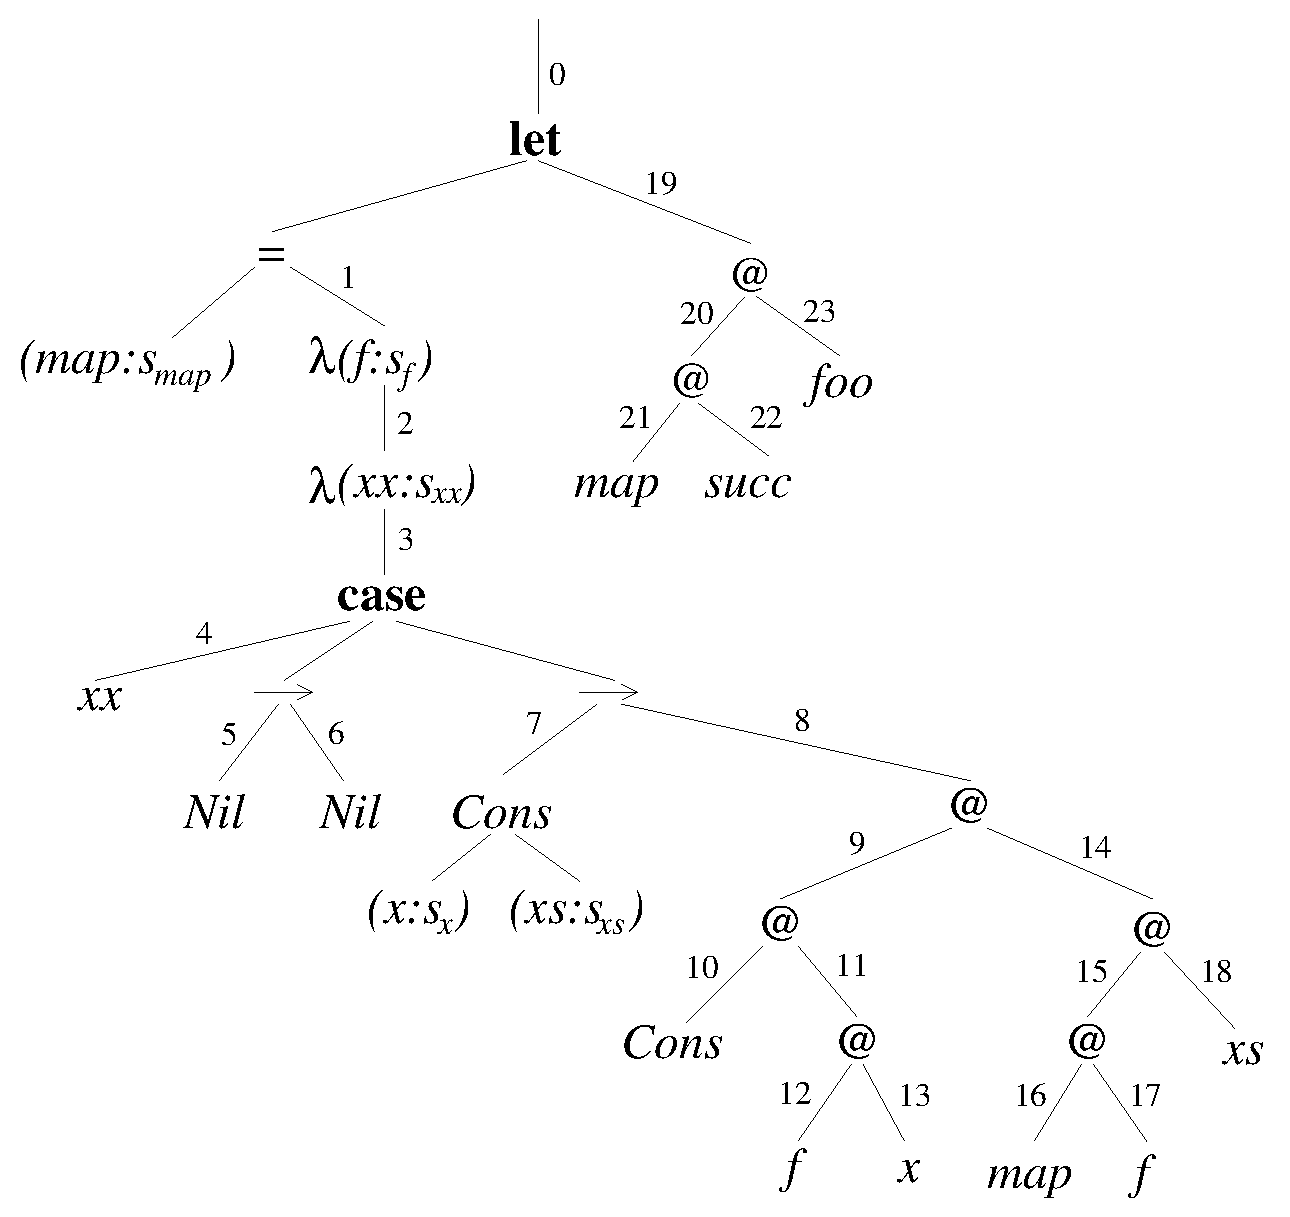
\includegraphics[scale=0.4]{3-Inference/fig/constraints/example-map}
\end{center}

\bigskip
\begin{tabular}{llllllll}
*0 	& $\sim \quad s_0$,	& $s_{19}$	&	& \quad $=$	& $\emptyset$ 
	\\[0.5ex]
*1 	& $\sim \quad s_{map}$, & $s_1, \ s_{16}$ &	& \quad	$=$	& $s_{f} \lfuna{e_{15a} \ c_{15}} s_{15}$, 
									& $s_f \lfuna{e_2 \ c_1} s_2$
	\\[0.5ex]
*2	& $\sim \quad s_f$,	& $s_{17}, \ s_{12}$ &	& \quad $=$	& $s_x \lfuna{e_{11a} \ c_{11}} s_{11}$
	\\[0.5ex]
*3	& $\sim \quad s_x$,	& $s_{13}, \ a_7$ &	& \quad $=$	& $\emptyset$
	\\[0.5ex]
*4	& $\sim \quad s_{xs}$,	& $s_{18}$	&	& \quad $=$	& $\iList \ r_7 \ a_7$
	\\[0.5ex]
*5	& $\sim \quad s_2$	& 		&	& \quad $=$	& $s_{xx} \lfuna{e_3 \ c_2} s_3$
	\\[0.5ex]
*6	& $\sim \quad s_3$,	& $s_6, \ s_8$	&	& \quad $=$	& $\iList \ r_6 \ a_6$
	\\[0.5ex]
*7	& $\sim \quad s_{xx}$,	& $s_4, \ s_5, \ s_7$ &	& \quad $=$	& $\iList \ r_5 \ a_5$,
									& $\iList \ r_7 \ a_7$
	\\[0.5ex]
*8	& $\sim \quad s_9$	&		&	& \quad $=$	& $s_{14} \lfuna{e_{8a} \ c_{3}} s_3$
	\\[0.5ex]
*9	& $\sim \quad s_{10}$	&		&	& \quad $=$	& $s_{11} \lfuna{e_{9a} \ c_{9}} s_9$,
									& $a_{10} \lfuna{\bot \ \bot} s_{10a}$
	\\[0.5ex]
*10	& $\sim \quad s_{10a}$	&		&	& \quad $=$	
							& \mc{2}{$s_{10b} \lfuna{\bot \ c_{10}} s_{10c}$}
	\\[0.5ex]
*11	& $\sim \quad s_{10b}$	&		&	& \quad $=$	& $List \ r_{10} \ a_{10}$
	\\[0.5ex]
*12	& $\sim \quad s_{10c}$	&		&	& \quad $=$	& $List \ r_{10} \ a_{10}$
	\\[0.5ex]
*13	& $\sim \quad s_{15}$	&		&	& \quad $=$	& $s_{xs} \lfuna{e_{14a} \ c_{14}} s_{14}$
	\\[0.5ex]
\ !0	& $\sim \quad e_0$	&		&	& \quad $\tme$	& $e_1 \lor e_{19}$
	\\[0.5ex]
\ !1	& $\sim \quad e_3$	&		&	& \quad $\tme$	& $\iReadH \ s_{\ixx} \lor e_6 \lor e_8$
	\\[0.5ex]
\ !2	& $\sim \quad e_8$	&		&	& \quad $\tme$	& $e_9 \lor e_{14} \lor e_{8a}$
	\\[0.5ex]
\ !3	& $\sim \quad e_9$	&		&	& \quad $\tme$	& $e_{10} \lor e_{11} \lor e_{9a}$
	\\[0.5ex]
\ !4	& $\sim \quad e_{11}$	&		&	& \quad $\tme$	& $e_{12} \lor e_{13} \lor e_{11a}$
	\\[0.5ex]
\ !5	& $\sim \quad e_{14}$	&		&	& \quad $\tme$	& $e_{15} \lor e_{18} \lor e_{14a}$
	\\[0.5ex]
\ !6	& $\sim \quad e_{15}$	&		&	& \quad $\tme$	& $e_{16} \lor e_{17} \lor e_{15a}$
	\\[1ex]
\$1	& $\sim \quad c_1$	&		&	& \quad $\tme$	& $\imap : s_{\imap}$
	\\[0.5ex]
\$2	& $\sim \quad c_2$	&		&	& \quad $\tme$	& $\imap : s_{\imap} \lor f : s_f$
	\\[0.5ex]
\$3	& $\sim \quad c_{10}$	&		&	& \quad $\tme$	& $x : a_{10}$
\end{tabular}


\pagebreak{}
\section{Constraint reduction}
\label{Inference:Reduction}

Our immediate goal is to determine a type for $\imap$. However, the equivalence class corresponding to $s_{\imap}$ currently contains two different type expressions. Although union typing systems \cite{dunfield:intersections-and-unions} provide a join operator on value types, we do not consider these systems here and will instead take the standard approach of unifying all the types in a particular equivalence class. Unifying all types corresponds to a ML style system, which is usually expressive enough for our needs. We will consider union typing again in \S\ref{Evaluation:Limitations:blocked-regions}.

The unification of types may generate more constraints. These new constraints must be added back to the graph, possibly resulting in more unifications, which may generate more constraints, and so on. In DDC we call this process \emph{grinding} the graph, and we take this to include performing unifications as well as reducing type class constraints and compound effects. 

\subsection{Constraint entailment}
We use entailment rules to describe operations on constraint sets. Entailment rules have the form $P \vvdash Q$, where $P$ and $Q$ are both sets. $P \vvdash Q$ can be read: ``$P$ entails $Q$'', or perhaps ``$P$ produces $Q$''. If we have a constraint set $R$ and a rule $P \vvdash Q$ where $P \subseteq R$, then we can replace the constraints $P$ in $R$ by the new constraints $Q$. Any variables present in $P$ match the corresponding types in $R$. For example, we could apply transitivity rule:

\begin{tabbing}
MMM \= MMMMMMM \= MMMMMMMMMMMMMMMMMM \kill
	\> (trans)	 \> $\{s_1 = s_2, \ s_2 = s_3 \}$ \\
	\> \qq $\vvdash$ \> $\{ s_1 = s_2, \ s_2 = s_3, \ s_1 = s_3 \}$
\end{tabbing}

To the following constraint set:

\code{
	$\{ s_{a} = s_{b}, \ s_{b} = \iInt \ r_1 \}$
}

to get:

\code{
	$\{ s_{a} = s_{b}, \ s_{b} = \iInt \ r_1, \ s_{a} = \iInt \ r_1 \}$
}


When we apply an entailment rule $P \vvdash Q$, we take any variables present in $Q$ but not $P$ or $R$ to be fresh.

Note that our entailment rules are expressed as operations on constraint sets, not on type graphs. To apply a rule to the type graph we must imagine it being converted to a constraint set and back again. As discussed in \S\ref{Inference:Constraints:sets-and-equiv-classes} the two forms are not totally equivalent, but the fact that we lose information when converting a constraint set to a type graph will only matter when we come come to discuss type error messages in \S\ref{inference:errors}. We use the graph representation until then as it is more compact and simplifies the presentation.

\clearpage{}
\subsection{Unification}


The entailment rules for unification are:

\begin{tabbing}
MMM \= MMMMMMM \= MMMMMMMMMMMMMMMMMM \kill
	\> (unify fun)	 \> $\{ \ s = a_1 \lfuna{e_1 \ c_1} b_1, \ s = a_2 \lfuna{e_2 \ c_2} b_2 \ \}$ \\
	\> \qq $\vvdash$ \> $\{ \ s = a_1 \lfuna{e_1 \ c_1} b_1, \ a_1 = a_2, \ b_1 = b_2, \ e_1 = e_2, \ c_1 = c_2 \ \}$	
\end{tabbing}

\begin{tabbing}
MMM \= MMMMMMM \= MMMMMMMMMMMMMMMMMM \kill
	\> (unify data)	 \> $\{ \ s = T_1 \ \ov{a}, \ s = T_1 \ \ov{b} \ \}$	\\[1ex]
	\> \qq $\vvdash$ \> $\{ \ s = T_1 \ \ov{a}, \ \ov{a = b} \ \}$
\end{tabbing}

The first rule is applicable when there are two function type constraints on a particular variable $s$. Applying the rule causes the second constraint to be discarded, while generating four new ones. These new constraints equate the type variables for the argument, return value, effect and closure of each function. The second rule is similar.

When we come to add a constraint like $a_1 = a_2$ to our type graph, if the two variables are already in the same equivalence class then we just ignore the constraint. If they are in separate classes then we add all the variables and types in the first one to the second, and delete the first (or \emph{vice-versa}). For example, our graph for $\imap$ includes the following:

\bigskip
\qq\qq
\begin{tabular}{lllllll}
*1 	& $\sim \quad s_{map}$, & $s_1, \ s_{16}$ &		
	& \quad	$=$	& $s_{f} \lfuna{e_{15a} \ c_{15}} s_{15}$, 
			& $s_f \lfuna{e_2 \ c_1} s_2$
\\[0.5ex]
*2	& $\sim \quad s_f$,	& $s_{17}, \ s_{12}$ &		& \quad $=$	& $s_x \lfuna{e_{11a} \ c_{11}} s_{11}$
\\[0.5ex]
*5	& $\sim \quad s_2$	& 		&		& \quad $=$	& $s_{xx} \lfuna{e_3 \ c_2} s_3$
\\[0.5ex]
*13	& $\sim \quad s_{15}$	&		&		& \quad $=$	& $s_{xs} \lfuna{e_{14a} \ c_{14}} s_{14}$
\\[0.5ex]
\ !7	& $\sim \quad e_{15a}$	& 		&		& \quad $\tme$	& $\bot$ 
\\[0.5ex]
\ !8	& $\sim \quad e_{2}$	& 		&		& \quad $\tme$	& $\bot$ 
\\[0.5ex]
\$1	& $\sim \quad c_1$	&		&		& \quad $\tme$	& $\imap : s_{\imap}$
\\[0.5ex]
\$4	& $\sim \quad c_{15}$	&		&		& \quad $\tme$ 	& $\bot$
\end{tabular}
\bigskip

Applying the unification rule to *1 allows us to delete the first function type, while generating the new constraints $s_f = s_f$, $s_{15} = s_2$, $e_{15a} = e_2$ and $c_{15} = c_1$. We can safely discard the trivial identity $s_f = s_f$. 

To add $s_{15} = s_2$ back to the graph we add the elements of *5 to *13 and discard *5. Likewise, to add $e_{15a} = e_2$ we will add the elements of !7 to !8 and delete !7. This yields:
\qq\qq
\begin{tabbing}
MMMMM 	\= MM 	\= MMMMM 		 	\= MMMMMM 		\= MMx \= MMM \= MMM \kill
	\> *1	\> $\sim \quad s_{map}$,	\> $s_1, \ s_{16}$ 	
		\> $\quad =$			\> $s_{f} \lfuna{e_2 \ c_1} s_{2}$ 
	\\
	\> *2	\> $\sim \quad s_f$,		\> $s_{17}, \ s_{12}$
		\> $\quad =$			\> $s_x \lfuna{e_{11a} \ c_{11}} s_{11}$ 
	\\
	\> *13	\> $\sim \quad s_{15}$,		\> $s_{2}$		
		\> $\quad =$			\> $s_{xs} \lfuna{e_{14a} \ c_{14}} s_{14},$
						 \  $s_{xx} \lfuna{e_3 \ c_2} s_3$ 
	\\
	\> \ !8	\> $\sim \quad e_2$, 	 	\> $e_{15a}$		
		\> $\quad \tme$			\> $\bot \lor \bot$ 
	\\
	\> \$1	\> $\sim \quad c_{1},$		\> $c_{15}$
		\> $\quad \tme$ 		\> $\imap : s_{\imap} \lor \bot$
\end{tabbing}

Note that when there are multiple types in a value type equivalence class we separate them by a comma. On the other hand, multiple types in an effect or closure equivalence class are separated by $\lor$. This follows naturally from the fact that constraints on value types are always expressed with =, but constraints on effects and closures are always expressed with $\tme$. Using the definition of $\lor$ we can then go on to simplify $\bot \lor \bot$ to just $\bot$. Note that in the constraint set representation this simplification isn't needed. If we have both $e_1 \tme \bot$ and $e_1 \tme \bot$, then putting these constraints in a set automatically `merges' them.

The application of (unify fun) to *1 has caused a new type to be added to *1. We keep applying our unification rules until no further progress can be made, and when this is done we have:

\bigskip
\qq
\begin{tabular}{llllllll}
*0 	& $\sim \quad s_0$,	& $s_{19}$	&		& \quad $=$	& $\bot$ 
	\\[0.5ex]
*1 	& $\sim \quad s_{map}$, & $s_1, \ s_{16}$ &		& \quad	$=$	& $s_f \lfuna{e_2 \ c_1} s_{15}$
	\\[0.5ex]
*2	& $\sim \quad s_f$,	& $s_{17}, \ s_{12}$ &		& \quad $=$	& $s_x \lfuna{e_{11a} \ c_{11}} s_{11}$
	\\[0.5ex]
*3	& $\sim \quad s_x$,	& $s_{13}, \ a_7, \ a_5$ & 	& \quad $=$	& $\bot$
	\\[0.5ex]
*6	& $\sim \quad s_3$,	& $s_6, \ s_8, s_{14}, s_{10b}, s_{10c}$	
				&	& \quad $=$	& $\iList \ r_6 \ s_{11}$
	\\[0.5ex]
*7	& $\sim \quad s_{xx}$,	& $s_4, \ s_5, \ s_7, s_{xs}, s_{18}$	
							&	& \quad $=$	& $\iList \ r_5 \ s_x$
	\\[0.5ex]
*9	& $\sim \quad s_{10}$	&		&		& \quad $=$	& $s_{11} \lfuna{e_{9a} \ c_9} s_{10a}$
	\\[0.5ex]
*10	& $\sim \quad s_{10a}$	& $s_9$		&		& \quad $=$	& $s_3 \lfuna{e_{8a} \ c_3} s_3$
	\\[0.5ex]
*13	& $\sim \quad s_{15}$, 	& $s_{2}$	&		& \quad $=$	& $s_{xx} \lfuna{e_3 \ c_2} s_3$
	\\[0.5ex]
*14	& $\sim \quad s_{11}$,	& $a_{10}, \ a_6$ &		& \quad $\tme$	& $\bot$
	\\
\%0	& $\sim \quad r_5,$	& $r_7$ 
	\\
\%1	& $\sim \quad r_6,$	& $r_{10}$ 
	\\
\ !0	& $\sim \quad e_0$	&		&		& \quad $\tme$	& $e_1 \lor e_{19}$
	\\[0.5ex]
\ !1	& $\sim \quad e_3,$	& $e_{14a}$	&		& \quad $\tme$	& $\iReadH \ s_{xx} \lor e_6 \lor e_8$
	\\[0.5ex]
\ !2	& $\sim \quad e_8$	&		&		& \quad $\tme$	& $e_9 \lor e_{14} \lor e_{8a}$
	\\[0.5ex]
\ !3	& $\sim \quad e_9$	&		&		& \quad $\tme$	& $e_{10} \lor e_{11} \lor e_{9a}$
	\\[0.5ex]
\ !4	& $\sim \quad e_{11}$	&		&		& \quad $\tme$	& $e_{12} \lor e_{13} \lor e_{11a}$
	\\[0.5ex]
\ !5	& $\sim \quad e_{14}$	&		&		& \quad $\tme$	& $e_{15} \lor e_{18} \lor e_{3}$
	\\[0.5ex]
\ !6	& $\sim \quad e_{15}$	&		&		& \quad $\tme$	& $e_{16} \lor e_{17} \lor e_{2}$
	\\[0.5ex]
\ !7	& $\sim \quad e_2,$	& $e_{15a}$	&		& \quad $\tme$	& $\bot$
	\\[1ex]
\$1	& $\sim \quad c_1$	&		&		& \quad $\tme$	& $\imap : s_{\imap}$
	\\[0.5ex]
\$2	& $\sim \quad c_2$	&		&		& \quad $\tme$	& $\imap : s_{\imap} \lor f : s_f$
	\\[0.5ex]
\$3	& $\sim \quad c_{10}$	&		&		& \quad $\tme$	& $x : a_{10}$

\end{tabular}


%--
\subsection{Head read}

When unification is complete we have a constraint $s_{xx} = \iList \ r_5 \ s_x$ in *7. This allows us to reduce the $\iReadH s_{xx}$ effect in !1 that was generated by the case-expression in the original program. In DDC we call the process of reducing effect types or type class constraints \emph{crushing}.

The entailment rule for $\iReadH$ is :
\begin{tabbing}
MMM \= MMMMMMM \= MMMMMMMM \= MMMMM \kill
	\> (read head)		\> $\{ \ e \tme \iReadH \ s,$ 	\> $s = T \ r \ \ov{s} \ \}$ \\
	\> \qq $\vvdash$	\> $\{ \ e \tme \iRead \ r,$	\> $s = T \ r \ \ov{s} \ \}$	
\end{tabbing}
This says that the effect of reading the primary region of a data type can be reduced to a simple read of that region once the region is known. This lets us reduce:
\qq\qq
\begin{tabbing}
MMMMM 	\= MM 	\= MMMMM 	\= MMMMMMMMMM 		\= MMx \= MMM \= MMM \kill
	\> *7	\> $\sim \quad s_{xx}$,	\> $s_4, \ s_5, \ s_7, \ s_{xs}, \ s_{18}$	
		\> \quad $=$		\> $\iList \ r_5 \ s_x$
	\\
	\> \ !1	\> $\sim \quad e_3,$	\> $e_{14a}$		
		\> \quad $\tme$		\> $\iReadH \ s_{xx} \lor e_6 \lor e_8$ 
\end{tabbing}
\vspace{-1em}
to:
\qq\qq
\begin{tabbing}
MMMMM 	\= MM 	\= MMMMM 	\= MMMMMMMMMM 		\= MMx \= MMM \= MMM \kill
	\> *7	\> $\sim \quad s_{xx}$,	\> $s_4, \ s_5, \ s_7, \ s_{xs}, \ s_{18}$	
		\> \quad $=$	\> $\iList \ r_5 \ s_x$
	\\
	\> \ !1	\> $\sim \quad e_3,$	\> $e_{14a}$		
		\> \quad $\tme$	\> $\iRead \ r_5 \lor e_6 \lor e_8$ 
\end{tabbing}

Recall that when applying an entailment rule, we must imagine the type graph being converted to a constraint set and back. The two equivalence classes *7 and !1 correspond to the set:

\code{
	$\{$	
	&  $s_{xx} = s_4$,	& $s_{xx} = s_5$,		& $s_{xx} = s_7$,	& $s_{xx} = s_{xs}$, \\
	& $s_{xx} = s_{18}$,	& $s_{xx} = \iList \ r_5 \ s_x$,&			& \\
	& $e_3 = e_{14a}$,	& $e_3 \tme \iReadH \ s_{xx}$,	& $e_3 \tme e_6$,	& $e_3 \tme e_8$ 
	& $\}$
}

Expressing the graph in this form separates out the constraints $e_3 \tme \iReadH \ s_{xx}$ and $s_{xx} = \iList \ r_5 \ s_x$, which match the premise of the (read head) rule.

\clearpage{}
\section{Generalisation}
\label{inference:generalisation}

When no more types can be unified, and no more effects or type class constraints can be reduced, the graph is said to be in \emph{normal form}. We can now extract the type for $\imap$ from our graph and generalise it into a type scheme.

In DDC we refer to the complete process of building a type scheme from the information in the type graph as ``generalisation''. This process is broken down into several stages, summarised below. Note that in a concrete implementation, several of these stages can performed at the same time. For example, checking for loops through the constraints can be done while tracing them, as tracing corresponds to a simple reachability analysis.

\bigskip
\qq
\begin{tabular}{lll}
	1. & Tracing:		& isolate the type information of interest. \\
	2. & Loop checking:	& check for infinite value type errors. \\
	3. & Packing:		& pack the graphical constraints into ``flat'' form. \\
	4. & Loop breaking:	& break loops through effect and closure constraints. \\
	5. & Cleaning:		& discard non-interesting effect and closure variables. \\
	6. & Quantification:	& introduce type quantifiers. 
\end{tabular}


% ---------------------------------------------------------
\subsection{Tracing}
The first step is to trace out the section of graph that is reachable from the type variable we're interested in. For this example we're interested in $\imap$ and all equivalence classes except *0 are reachable from $s_{\imap}$. This process makes a copy of the information present in the ``global'' graph, and the operations described in the rest of this section are performed on the copy. 


% ---------------------------------------------------------
\subsection{Loop checking}
We now check for loops through the value type portion of the copied sub-graph. A classic example of a program with a looping type is:

\qq\qq
\begin{tabular}{ll}
	$x$	& $= \iCons \ x \iNil$
\end{tabular}

where $\iCons$ and $\iNil$ have the following types:

\code{
	$\iNil$	& $:: \forall r \ a. \iList \ r \ a$ \\

	$\iCons$	
		& $:: \forall r \ a \ c. \ a \to \iList \ r \ a \lfuna{c} \iList \ r \ a$ \\
		& $\rhd \ c \tme x : a$
}



After slurping and grinding constraints, this program has the following graph:
\qq\qq
\begin{tabbing}
MMMMM 	\= MM 	\= MMMMM 	\= MMMMMMMMMM 		\= MMx \= MMM \= MMM \kill
	\> \ *1	\> $\sim \quad s_x,$	\> $s_1, \ s_4, \ a_3, \ a_5$	\> \quad $=$	\> $\iList \ r_3 \ s_x$ \\
	\> \ *2	\> $\sim \quad s_2$,	\>				\> \quad $=$	\> $s_5 \lfuna{e_1 \ c_1} s_x$ \\
	\> \ *3	\> $\sim \quad s_3$,	\> $s_{\iCons}$			\> \quad $=$	\> $s_4 \lfuna{e_2 \ c_2} s_2$ \\
	\> \ *4 \> $\sim \quad s_5$,	\> 				\> \quad $=$	\> $\iList \ r_3 \ s_x$ \\
	\> \ \$1 \> $\sim \quad c_3$,	\> $c_1$			\> \quad $\tme$	\> $x : s_x$ \\
	\> \ \%1 \> $\sim \quad r_3$,	\> $r_5$ 
\end{tabbing}


The loop is through equivalence class *1. We cannot produce a flat, non-graphical type for $s_x$ because if we tried to solve its constraint our algorithm would diverge:

\code{
		& $s_x$	& $= \iList \ r_3 \ s_x$ \\
 $\equiv$	& $s_x$ & $= \iList \ r_3 \ (\iList \ r_3 \ s_x)$ \\
 $\equiv$	& $s_x$ & $= \iList \ r_3 \ (\iList \ r_3 \ (\iList \ r_3 \ s_x))$ \\
 $\equiv$	& \dots 
}

\bigskip
Unlike \cite{cardone:recursive-types} we do not attempt to handle recursive value types, so we flag them as errors instead. This is common to other compilers such as GHC, which would emit a message ``cannot construct infinite type''. Note that loops through the effect or closure portions of a type graph are \emph{not} counted as errors. We deal with these in \S\ref{Inference:Generalisation:loop-breaking}.


% ---------------------------------------------------------
\subsection{Packing}
Packing is the process of converting a set of individual type constraints into the normalised form of \ref{inference:language:normal-types}. When we pack the constraints from our $\imap$ example into this form we have:

\bigskip
\begin{tabular}{llllll}
	$s_{\imap}$	
	& \mc{3}{$= (s_x \lfuna{e_{11a} \ c_{11}} s_{11}) 
			\lfuna{e_2 \ c_1} \iList \ r_5 \ s_x 
			\lfuna{e_3 \ c_2} \ \iList \ r_6 \ s_{11}$} 
	\\[1ex]
	& $\rhd$ & $e_3$ 	& $\tme \ \iRead r_5 \lor e_6 \lor e_8$	\\
	& \ ,	 & $e_8$	& $\tme \ e_9 \lor e_{14} \lor e_{8a}$ \\
	& \ ,  	 & $e_9$	& $\tme \ e_{10} \lor e_{11} \lor e_{9a}$ \\
	& \ ,	 & $e_{11}$	& $\tme \ e_{12} \lor e_{13} \lor e_{11a}$ \\
	& \ ,	 & $e_{14}$	& $\tme \ e_{15} \lor e_{18} \lor e_3$ \\
	& \ ,	 & $e_{15}$	& $\tme \ e_{16} \lor e_{17} \lor e_{2}$ \\
	& \ , 	 & $c_{1}$	& $\tme \ \imap : (s_x \lfuna{e_{11a} \ c_{11}} s_{11}) 
							\lfuna{e_2 \ c_1} \iList \ r_5 \ s_x 
							\lfuna{e_3 \ c_2} \ \iList \ r_6 \ s_{11}$ \\
	& \ , 	 & $c_{2}$	& $\tme \  \imap : (s_x \lfuna{e_{11a} \ c_{11}} s_{11}) 
							\lfuna{e_2 \ c_1} \iList \ r_5 \ s_x 
							\lfuna{e_3 \ c_2} \ \iList \ r_6 \ s_{11}$ \\
	&	&		& $\ \ \ \ \ \ \ \lor \ f : s_x \lfuna{e_{11a} \ c_{11}} s_{11}$
\end{tabular}

\bigskip
Although the body of this type is now in the familiar form, there is still a hash of effect and closure constraints. However, notice that there is only one use each of the variables $e_8, \ e_9, \ e_{11}, \ e_{14}$ and $e_{15}$, and they are not mentioned in the body of this type. From a compiler optimisation point of view, the only effect information that we need to preserve is the manifest effect of each function arrow. The fact that, say, $e_3$ includes $e_8$ and $e_8$ includes $e_9$ does not matter, as long as all of the appropriate variables are reachable from $e_3$.

This means that we can inline the constraints on $e_8$, $e_9$ and so on into the constraint for $e_3$. We can also use the closure trimming process discussed in \S\ref{System:Closure:trimming} to simplify the constraints for $c_1$ and $c_2$. This produces:

\bigskip
\code{	
	$s_{\imap}$	
	& \mc{3}{$= (s_x \lfuna{e_{11a} \ c_{11}} s_{11}) 
			\lfuna{e_2 \ c_1} \iList \ r_5 \ s_x 
			\lfuna{e_3 \ c_2} \ \iList \ r_6 \ s_{11}$} 
	\\[1ex]
	& $\rhd$ & $e_3$ 	& $\tme \ \iRead r_5 \lor e_6 \lor e_8 \lor e_9 \lor e_{14} \lor e_{8a}$ \\
	&	 &		& $ \qq \qq \ \ \ \lor \ e_{10} \lor e_{11} \lor e_{9a} 
					\lor e_{12} \lor e_{13} \lor e_{11a}$ \\
	&	 &		& $ \qq \qq \ \ \ \lor \ e_{15} \lor e_{18} \lor e_3 
					\lor e_{16} \lor e_{17} \lor e_{2}$ \\
	& \ , 	 & $c_{1}$	& $\tme \ \imap  : c_1$ \\
	& \ , 	 & $c_{2}$	& $\tme \  \imap : c_1 \lor \ f : c_{11}$
}


% ---------------------------------------------------------
\subsection{Loop breaking}
\label{Inference:Generalisation:loop-breaking}
As discussed in \S\ref{System:Effects:recursive}, we can use the lattice structure of effects and closures to break loops through effect and closure constraints. If the type of a particular value variable contains looping constraints, then breaking these loops makes the type simpler, and allows it to be exported to the core language. The following diagram shows a loop through the effect portion of the type for $\imap$, as it was after the first stage of packing:

\begin{center}
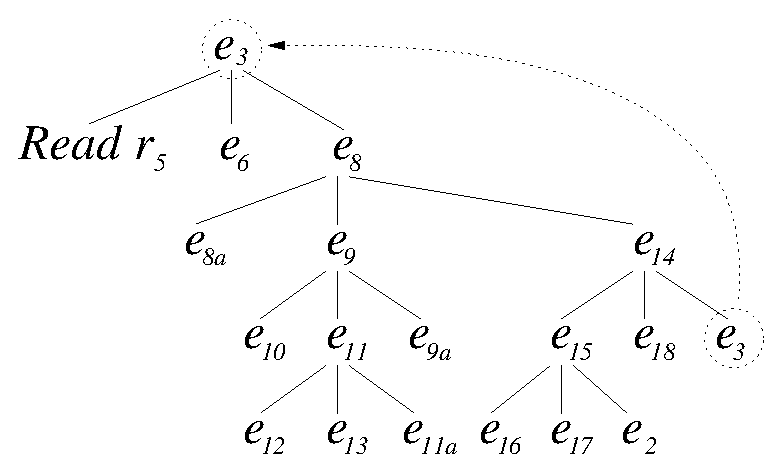
\includegraphics[scale=0.5]{3-Inference/fig/generalisation/loop-effect}
\end{center}

Notice how the structure of this effect graph echos the original abstract syntax tree for $\imap$. In the effect graph we can see two branches, headed by $e_9$ and $e_{14}$, corresponding to the two alternatives of the original case expression. We can also see the recursive call via $e_3$. $\imap$ applies itself, so the effect of $\imap$ includes the effect of $\imap$. Similarly, $\imap$ references itself, so the closure of $\imap$ includes the closure of $\imap$.

However, although recursion in the function's \emph{definition} serves a useful purpose, the fact that its effect and closure is also recursive is not exploited by our analysis. We need to retain the set of effects caused by an application of $\imap$, that is, the effects reachable from $e_3$, but this information would not be lost if we substituted $\bot$ for its recursive occurrence. Finally, the constraints $e_3 \tme e_3$ and $c_1 \tme \imap : c_1$ are trivially satisfied, so can be discarded. This leaves us with:

\bigskip
\qq
\begin{tabular}{llll}
	$s_{\imap}$	
		& \mc{3}{$= (s_x \lfuna{e_{11a} \ c_{11}} s_{11}) 
				\lfuna{e_2 \ c_1} \iList \ r_5 \ s_x 
				\lfuna{e_3 \ c_2} \ \iList \ r_6 \ s_{11}$} 
		\\[1ex]
		& $\rhd$ & $e_3$ 	& $\tme \ \iRead r_5 \lor e_6 \lor e_8 \lor e_9 \lor e_{14} \lor e_{8a}$ \\
		&	 &		& $ \qq \qq \ \ \ \lor \ e_{10} \lor e_{11} \lor e_{9a} \lor e_{12} \lor e_{13} \lor e_{11a}$ \\
		&	 &		& $ \qq \qq \ \ \ \lor \ e_{15} \lor e_{18} \lor \bot \lor e_{16} \lor e_{17} \lor e_{2}$ \\
		& \ , 	 & $c_{2}$	& $\tme \  \imap : c_1 \lor \ f : c_{11}$
\end{tabular}


% ---------------------------------------------------------
\subsection{Cleaning}
There are still a large number of effect and closure variables in our type that don't provide any useful information. For example, $e_6$ is the effect of evaluating the variable $\iNil$, but evaluating a variable doesn't have a visible effect. Also consider $e_9$, the effect of evaluating $\iCons \ (f \ x)$. The evaluation of $(f \ x)$ itself has the effect $e_{11}$, which is interesting because it depends on the function argument passed to map, but the partial application of $\iCons$ to the result does not have an effect, so is boring. In any event, the constraint on $e_3$ already contains $e_{11}$, so it doesn't need to include $e_9$ as well.

We define boring effect and closure variables to be the ones that are completely unconstrained. Such variables are not mentioned in the type environment, in a parameter of the type being generalised, or on the left of an (in)equality. If a variable is in the type environment then it depends on a definition in a higher scope of the program. In this case, a more interesting type may be unified into the variable later in the inference process. If it is mentioned in a parameter type then it may be different for each application of the function. If it is on the left of an (in)equality then it depends on other types. For our example, $e_{11a}, \ c_{11}, \ e_{3}$ and $c_{2}$ are interesting, and the rest are boring. We substitute $\bot$ for boring variables, then use the definition of $\lor$: 

\bigskip
\qq
\begin{tabular}{llll}
	$s_{\imap}$	
		& \mc{3}{$= (s_x \lfuna{e_{11a} \ c_{11}} s_{11}) 
				\lfun \iList \ r_5 \ s_x 
				\lfuna{e_3 \ c_2} \ \iList \ r_6 \ s_{11}$} 
		\\[1ex]
		& $\rhd$ & $e_3$ 	& $\tme \ \iRead r_5 \lor e_{11a}$ \\
		& \ , 	 & $c_{2}$	& $\tme \ f : c_{11}$
\end{tabular}


% ---------------------------------------------------------
\subsection{Quantification}
We can now add quantifiers to our type and create a type scheme. There are several restrictions as to what variables can be quantified, which we will recall in a moment, but for this example none apply. After quantification we have:

\bigskip
\qq
\begin{tabular}{llll}
	$s_{\imap}$	
		& \mc{3}{$= \forall s_x \ s_{11} \ r_5 \ r_6 \ e_{11a} \ c_{11} \ e_3 \ c_2$} \\[1ex]
		& \mc{3}{$. \ \ \ \ (s_x \lfuna{e_{11a} \ c_{11}} s_{11})
				\lfun \iList \ r_5 \ s_x \lfuna{e_3 \ c_2} \ \iList \ r_6 \ s_{11}$} 
		\\[1ex]
		& $\rhd$ & $e_3$ 	& $\tme \ \iRead \ r_5 \lor e_{11a}$ \\
		& , 	 & $c_{2}$	& $\tme \ f : c_{11}$
\end{tabular}

\bigskip
We will also rewrite the quantified variables to use more familiar names:

\qq
\begin{tabular}{llll}
	$s_{\imap}$	
		& \mc{3}{$= \forall a \ b \ r_1 \ r_2 \ e_1 \ e_2 \ c_1 \ c_2$} \\[1ex]
		& \mc{3}{$. \ \ \ \ (a \lfuna{e_1 \ c_1} b)
				\lfun \iList \ r_1 \ a  \lfuna{e_2 \ c_2} \ \iList \ r_2 \ b$} 
		\\[1ex]
		& $\rhd$ & $e_2$ 	& $\tme \ \iRead \ r_1 \lor e_{1}$ \\
		& , 	 & $c_2$	& $\tme \ f : c_{1}$
\end{tabular}

\medskip
At this stage we could also apply the the effect masking rules from \S\ref{System:Effects:masking} and \S\ref{System:Closure:masking}, though none apply in this example. Once generalisation is complete we update the $s_{\imap}$ equivalence class in the global graph so it contains this new type scheme.

\subsubsection{The non-generalisable variables}
There are several reasons why a particular type variable may not be permitted to be generalised. All but the first were discussed in the previous chapter.

Don't generalise:
\begin{enumerate}
\item	Variables free in the type environment. This is the standard restriction for Hindley-Milner
	type systems \cite{milner:type-polymorphism, damas:principle-type-schemes}. However, as we're
	performing type inference instead of type \emph{checking}, the real type environment is not
	close at hand. We instead use the method discussed in \S\ref{inference:ordering} to
	determine the value variables that are free in the binding whose type is being generalised.
	The types of these variables can be determined from the graph, and we hold their free type
	variables monomorphic. This achieves the same result.
	
\item	Dangerous type variables, which were discussed in \S\ref{System:Closure:dangerous} and 
	\S\ref{Inference:Language:dangerous-variables}. These are variables that appear free under
	type constructors whose regions are constrained to be mutable. Dangerous type variables must be
	held monomorphic to avoid the problem with polymorphic update that was discussed in \S\ref{System:Update}.

\item	Material region variables, which were discussed in \S\ref{System:Closure:non-material-regions}.
	Material regions correspond with objects that are shared between all uses of the variable
	whose type is being generalised. These must also be held monomorphic.
\end{enumerate}


% ---------------------------------------------------------
\subsection{Late constraints and post-inference checking}
\label{Inference:Generalisation:late-constraints}

The fact that mutability constraints influence what type variables are quantified introduces a slight complication into the inference process. The type inferencer might quantify a type variable while assuming that a particular region is constant, but later discover a mutability constraint that indicates it shouldn't have quantified. We refer to such mutability constraints as \emph{late} constraints. The following example demonstrates the problem:

\bigskip
\code{	\mc{2}{$\ilateFun \ ()$} \\
	\ $= \kdo$ 	& $\iref$	& $ = \inewRef \ \iid$		\\
			& $f$		& $ = \lambda(). \ireadRef \ \iref$ \\
			& \mc{2}{$\iwriteRef \ \iref  \ \isucc$}	\\
	 		& \mc{2}{$f \ ()$ \ ``\texttt{oh noes}''}
}

with

\code{	$\iid$ 	
		& $::$	& $\forall a. \ a \to a$ 	
	\\[1ex]
	$\isucc$
		& $::$		& $\forall r_1 \ r_2 \ e_1. \ \iInt \ r_1 \lfuna{e_1} \iInt \ r_2$	 \\
		& $\rhd$	& $e_1 \tme \iRead \ r_1$
	\\[1ex]
	$\inewRef$
		& $::$		& $\forall a \ r_1. \ a \to \iRef \ r_1 \ a$
	\\[1ex]
	$\ireadRef$
		& $::$		& $\forall a \ r_1 \ e_1. \iRef \ r_1 \ a \lfuna{e_1} a$ \\
		& $\rhd$	& $e_1 \tme \iRead \ r_1$
	\\[1ex]
	$\iwriteRef$
		& $::$		& $\forall a \ r_1 \ e_1 \ c_1. \iRef \ r_1 \ a \to a \lfuna{e_1 \ c_1} ()$ \\
		& $\rhd$	& $e_1 \tme \iWrite \ r_1$ \\
		& ,		& $c_1 \tme x : \iRef \ r_1 \ a$ \\
		& ,		& \mc{2}{$\iMutable \ r_1$}
}

From the types of $\inewRef$, $\ireadRef$ and $\iwriteRef$, we see that an object of type $\iRef \ r_1 \ a$ is only treated as mutable if we actually apply the $\iwriteRef$ function to it. If we only ever \emph{read} a reference, then there is no need to mark it as mutable or restrict the type of the contained value. However, with our $\ilateFun$ example, the type inferencer will only discover that $\iref$ is mutable when it processes the third line of the do-expression. If it considers the bindings in-order, and generalises the type of $\iref$ while assuming constancy, it will get:

\code{
	$\iref :: \forall a. \iRef \ r_1 \ (a \to a)$
}

\clearpage{}

with this scheme, the type of $f$ becomes:

\code{
	$f$	& $::$ 		& $ \forall b \ e_1 \ c_1. \ () \lfuna{e_1 \ c_1} b \to b$ \\
		& $\rhd$	& $e_1 \tme \iRead \ r_1$ \\
		& ,		& $c_1 \tme \iref : \iRef \ r_1 \ (b \to b)$
}

Later, the inferencer will discover the call to $\iwriteRef$, which places a mutability constraint on $r_1$ and invalidates the previous type scheme for $\iref$. Note that it is not safe to simply change the scheme for $\iref$ to a less general one ``on the fly'', because the old scheme was instantiated when inferring the type of $f$, and now that type is wrong as well. 

A simple solution is to wait until type inference is complete, re-generalise the types of all let-bound variables, and compare the resulting type schemes against the previously inferred ones. Waiting until inference is complete ensures that all the available mutability constraints have made their way into the type graph. If a newly generalised scheme is different to its original version, then a mutability constraint must have been added to the graph after the original was created. This is reported as an error.

This solution has the disadvantage of requiring the types of polymorphic mutable objects to be given explicitly as signatures. For example, although the following program will not cause a problem at runtime, it will be marked as erroneous:

\code{
	$\ifalseLate$ \\	
	\ $= \kdo$ 	& $\iref$	& $ = \inewRef \ \iid$		\\
			& \mc{2}{$\iwriteRef \ \iref  \ \isucc$}	\\
			& \mc{2}{$(\ireadRef \iref) \ 5$}
}

Adding a type signature ensures that the inferencer will treat $\iref$ as being mutable when its type is generalised:

\code{
	$\ifixedLate'$ \\
	\ $= \kdo$ 	& \mc{2}{$\iref :: \iRef \ r_1 \ (a \to a) \rhd \iMutable \ r_1$} \\
			& $\iref$	& $ = \inewRef \ \iid$		\\
			& \mc{2}{$\iwriteRef \ \iref  \ \isucc$}	\\
			& \mc{2}{$(\ireadRef \iref) \ 5$}
}

\bigskip
An alternate solution would be to re-generalise the type of $\iref$ at each instantiation point. If the newly generalised scheme was different to the previous one, then we could backtrack to original definition and re-type the subsequent program using the new scheme. We could also perform backtracking in a coarse grained manner, by doing the post-inference check as before, but re-typing the \emph{whole} program if any schemes were different. However, backtracking adds extra complexity, and we expect programs like the above to be rare, so we use the simpler non-backtracking solution in our implementation.

The BitC compiler also checks for the late constraint problem \cite{sridhar:type-inference-systems-language}. It does not backtrack, but performs the check during type inference proper. It also uses local heuristics to guess whether a particular variable is mutable, without performing complete inference. Before generalising the type of a variable it inspects how it is used later in the function. If the variable is updated locally, its type is generalised using this information. This is possible in BitC because the assignment operator $:=$ is baked into the language, instead of being defined in the standard libraries.



\clearpage{}
\section{Type directed projections}
\label{System:Projections}

In \S\ref{Intro:Update:broadcast} we discussed how references (and pointers) are used to update values within container structures, without knowledge of the surrounding container. We also discussed how they are used to update values that are shared by several different parts of the program, without needing information about how they are shared. On the other hand, in \S\ref{intro:ref-types} we saw how the use of ML style references can lead to a large amount of refactoring effort when writing programs. This is because the reference appears in the value types of terms that use them, and we must use an explicit function call to read a reference when we want the contained value.

The Disciple projection system provides a mechanism to create references on the fly, so we can use them for shared update without the need to change the structure of value types. The fact that we can provide this mechanism while still tracking enough information to perform compile type optimisations is the primary reason we have developed the type system discussed in this chapter. We also provide a separate name space associated with each type constructor, and  projection functions are placed in the name space corresponding to the type of value they project. This avoids the problem with Haskell style records, also discussed in \S\ref{Intro:Update:broadcast}, where the names of projection functions pollute the top-level scope of the program. In this thesis we restrict ourselves to associating namespaces with \emph{constructors} instead of general types. This is to avoid issues with overlapping types such as $\iList \ a$ and $\iList \ \iInt$. 

Projections are complementary to type classes. For example, when performing type inference for an expression like $\ishow \ x$, the variable $x$ may have a polymorphic type. As the instance function to use for $\ishow$ may be resolved at run time via a dictionary passing mechanism\footnote{At least it can in a mature compiler like GHC. Our prototype implementation does not yet support dictionary passing, though we are not aware of any barrier to adding it. }, the compiler itself will not know which instance function will be used. Due to this, the type of $\ishow$ in the class definition must be an upper bound of the types of all possible instances.

On the other hand, when performing type inference for the projection $x \ \odot \ \ifieldOne$, we require the type of $x$ to resolve to something that includes an outer constructor. We use this constructor to determine how to implement the projection of $\ifieldOne$. This in turn allows each of the projections named $\ifieldOne$ to return values of \emph{different} types.

% -----------------
\subsection{Default projections}
\label{System:Projections:default}

Consider the following data type definition. 

\code{
	$\kdata$ \ $\iVecTwo \ r \ a = \iVecTwo \ \{ \ x :: a; \ y :: a \ \}$
}

$x$ and $y$ are the field names of the constructor. In Haskell, this definition would introduce $x$ and $y$ as record selectors in the top level scope. In Disciple, we instead get two projections $\odot \ x$ and $\odot \ y$ that can be applied to values of type $\iVecTwo \ r \ a$, for any $r$ or $a$. As our type expressions may contain commas, we use a semicolon as a field separator instead of a comma.  Also, $\odot$ is an infix operator, and $\odot \ x$ is written \texttt{.x} in the concrete syntax. Here is an expression which uses the two projections:

\code{
	$\kdo$	
		& $\ivec$	& $= \iVecTwo \ 2.0 \ 3.0$ \\
		& $\iangle$	& $= \isqrt \ (\isquare \ \ivec \odot \ x + \isquare \ \ivec \odot \ y)$ \\
}

The projection operator $\odot$ binds more tightly than function application, so $\isquare \ \ivec \odot \ x$ should be read as $\isquare \ (\ivec \odot \ x)$. If we do not have a handy object of the required type then we can refer to the projection functions in a particular namespace directly with the $\&$ operator. For example, we could rewrite the above expression as:

\code{
	$\kdo$	& $\ivec$	& $= \iVecTwo \ 2.0 \ 3.0$ \\
		& $\iangle$	& $= \isqrt \ 		(\isquare \ (\iVecTwo\&x \ \ivec)$ \\ 	
		&		& \qq \qq \qq $ + \ 	(\isquare \ (\iVecTwo\&y \ \ivec))$ \\
}

The projections associated with field names are called \emph{default projections}. These are introduced automatically by the language definition. For $\iVecTwo$ the two projection functions are:

\code{
	$\iVecTwo \: \& \: x$	
		& $::$		& $\forall r_1 \ a. \ \iVecTwo \ r_1 \ a \lfuna{e_1} a$ \\
		& $\rhd$	& $e_1 = \iRead \ r_1$ 
	\\[1ex]
	\mc{3}{$\iVecTwo \: \& \: x \ \ (\iVecTwo \ x \ y) = x$}
	\\[3ex]
	$\iVecTwo \: \& \: y$	
		& $::$		& $\forall r_1 \ a. \ \iVecTwo \ r_1 \ a \lfuna{e_1} a$ \\
		& $\rhd$	& $e_1 = \iRead \ r_1$ 
	\\[1ex]
	\mc{3}{$\iVecTwo \: \& \: y \ \ (\iVecTwo \ x \ y) = y$}
}

This syntax is similar to the use of $::$ in C++ to define class methods. For example, the name of a method in a class named $\iVecTwo$ would be $\iVecTwo::x$. 

\clearpage{}
% ---------------------------
\subsection{Ambiguous projections and type signatures}
\label{System:Projections:ambiguous}

Ambiguous projections arise when we project a value whose type is not constrained to include an outer constructor. For example, the projections in the following code are ambiguous:

\code{
	$\itupleOfVec$ = $\lambda \ivec. \ (\ivec \ \odot \ x, \ \ivec \ \odot \ y)$ 
}

Without further information, the type of $\ivec$ in this code is just a variable. If our program included more than one data type that had an $x$ or $y$ field, then there would be no way of knowing which projection function to use. 

The programmer can resolve this problem by providing a type signature that constrains the type of $\ivec$. For example:

\code{
	\mc{2}{$\itupleOfVec :: \iVecTwo a \to (a, \ a)$} \\
	$\itupleOfVec$ = $\lambda \ivec. \ (\ivec \ \odot \ x, \ \ivec \ \odot \ y)$ 
}

Note that we do not need to provide region, effect or closure information in type signatures. The fact that this information is missing from the above signature can be determined from the kind of $\iVecTwo$, and it can be filled in by the type inference process. 

% ---------------------------
\subsection{Pull back projections}
\label{System:Projections:pull-back}

Pull back projections allow the programmer to create references to the fields of a record. For example, a reference to the $x$ field of our $\iVecTwo$ type can be created with $\ivec \: \odot_{\#} \: x$, pronounced ``$\ivec$ pull $x$''. If the type of $\ivec$ is $\iVecTwo \ r_1 \ a$ then the type of $\ivec \: \odot_{\#} \: x$ is $\iRef \ r_1 \ a$. If we imagine $\iRef$ types being equivalent to pointers in C, then $\ivec \: \odot_{\#} \: x$ has the same meaning as the C expression \texttt{\&(vec.x)}. The $:=_{\#}$ function (pronounced ``update ref'') is then used to update the value of the field. Note that $\ivec \: \odot_{\#} \: x$ and $:=_{\#}$ are written as \texttt{vec\#x} and \texttt{\#=} in the concrete syntax.

Here is the type of $:=_{\#}$

\code{
	$(:=_{\#})$  
		& $::$		& $\forall r_1 \ a. \ \iRef \ r_1 \ a \lfun a \lfuna{e_1 \ c_1} ()$ \\
		& $\rhd$ 	& $e_1 = \iWrite \ r_1$  \\
		& \ ,		& $c_1 = x : \iRef \ r_1$ \\
		& \ ,		& \mc{2}{$\iMutable \ r_1$}
}

Here is an example that creates a vector then updates one of its components:

\code{
	$\kdo$	& $\ivec$	& $= \iVecTwo \ 2.0 \ 3.0$ \\
		& $\iref$	& $= \ivec \: \odot_{\#} \: x$ \\
		& \dots \\
		& $\iref$	& $:=_{\#} \ 5.0$ \\
		& \dots \\
}

After the update statement has been executed, the projection $\ivec \ \odot \ x$ will return the value $5.0$ instead of $2.0$. Pull back projection functions can also be accessed directly. Here are the names and types of the pull back projections for the $x$ and $y$ fields:

\code{
	$\iVecTwo \: \& \:x_{\ipull}$	
		& $ :: \forall r_1 \ a. \ \iVecTwo \ r_1 \ a \fun \iRef \ r_1 \ a$  
	\\[1ex]
	$\iVecTwo \: \& \:y_{\ipull}$
		& $ :: \forall r_1 \ a. \ \iVecTwo \ r_1 \ a \fun \iRef \ r_1 \ a$ 
}

Note that the created reference shares the same region variable as the projected value. Also note that as $\iVecTwo$ only has a single data constructor, the functions $x_{\ipull}$ and $y_{\ipull}$ are pure. This is because when we evaluate an expression like $\ivec \: \odot_{\#} \: x$, we do not need to access the $\ivec$ object at all. We simply allocate a new reference that contains a pointer into it. This can be done based on the address of the $\ivec$ object, the object itself is not needed. For example, if we say:

\code{
	$\ivec$ 	& $:: \iVecTwo \ r_1 \ (\iFloat \ r_2) \ (\iFloat \ r_3)$  \\
	$\ivec$		& $= \iVecTwo \ 2.0 \ 3.0$
}

then we would have:

\code{
	$\iref$	& $:: \iRef \ r_1 \ (\iFloat \ r_2)$ \\
	$\iref$ & $= \ivec \: \odot_{\#} \: x$
}

which produces the following objects in the store:

\begin{center}
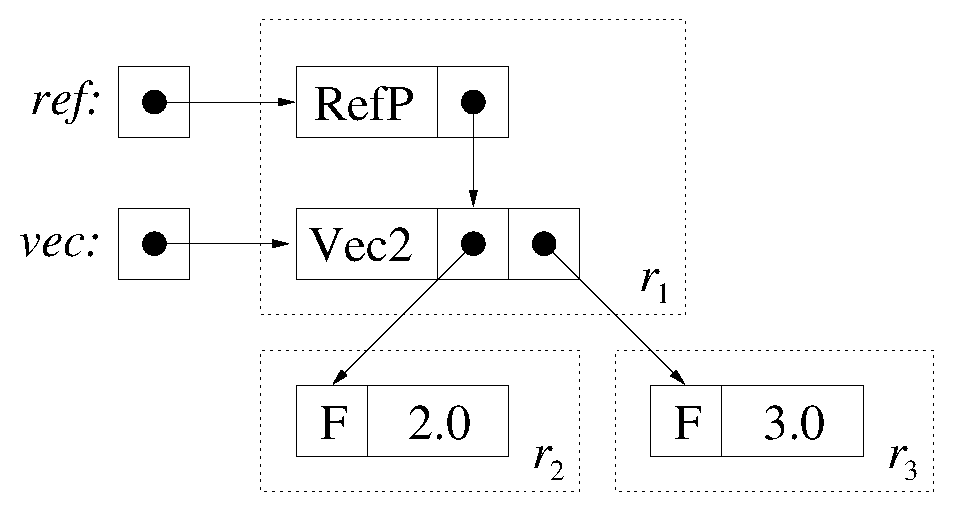
\includegraphics[scale=0.5]{2-System/fig/projections/pull-back}
\end{center}

We use the tag $\iRefP$ to record the fact that the $\iref$ object is a pull back reference that points into another object, as opposed to a regular ML style reference. When we execute the statement $\iref :=_{\#} 5.0$, it is the pointer inside the $\ivec$ object that is updated, not the $\iFloat$ object itself:

\begin{center}
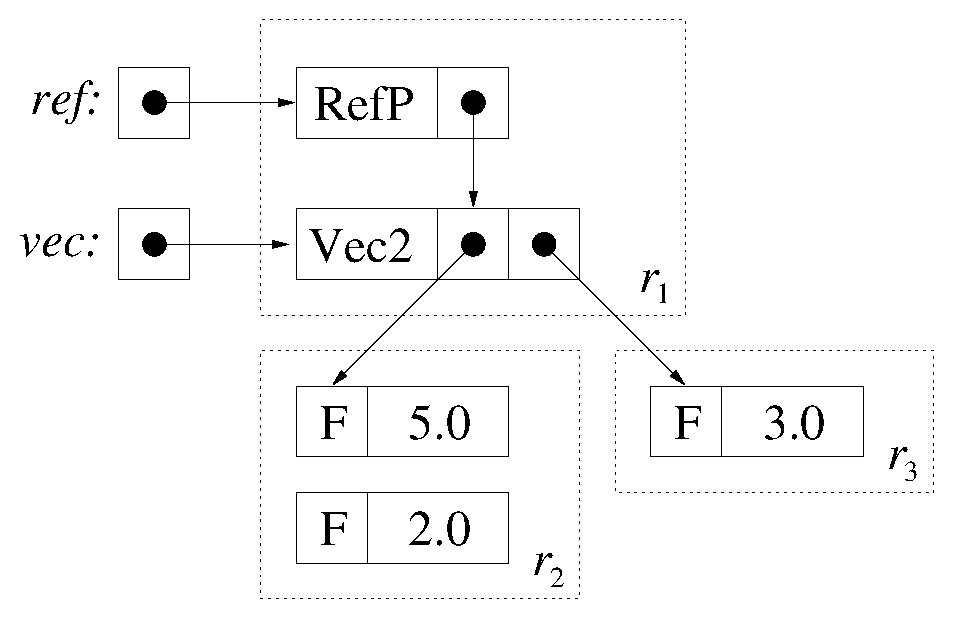
\includegraphics[scale=0.5]{2-System/fig/projections/pull-back-update}
\end{center}

This leaves the old $2.0$ object to be reclaimed by the garbage collector.

The benefit of this system over ML style references is that we are able to update data structures without needing $\iRef$ in their type definitions, which addresses the refactoring problem discussed in \S\ref{intro:ref-types}. Note that in the above diagram, both the $\iVecTwo$ and $\iRefP$ objects are in the same region, $r_1$. This means that when we use a function like $(:=_{\#})$ to update the vector via the reference, the vector object will also be marked as mutable.

Although we don't \emph{need} ML style references, Disciple does support them, and we can equally define:

\code{
	$\kdata$ \ $\iVecTwo \ r_1 \ a = \iVecTwo \ \{ \ x :: \iRef \ r_1 \ a; \ y :: \iRef \ r_1 \ a \ \}$
}

In this case we would construct a vector with:

\code{
	$\ivec$		& $:: \iVecTwo \ r_1 \ (\iFloat \ r_2) \ (\iFloat \ r_3)$ \\
	$\ivec$		& $= \iVecTwo \ (\iRef \ 2.0) \ (\iRef \ 3.0)$
}

This produces the following objects in the store:

\begin{center}
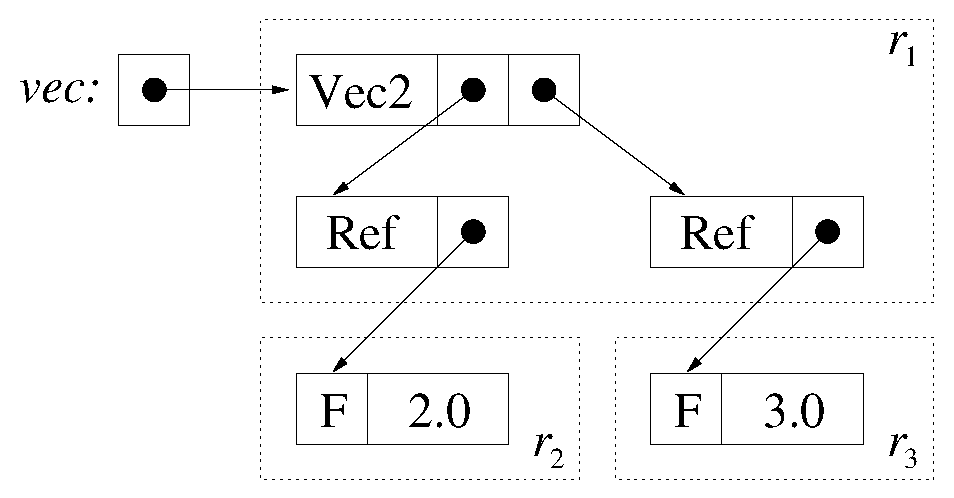
\includegraphics[scale=0.5]{2-System/fig/projections/vec-ref}
\end{center}

Here, the reference objects include the constructor tag $\iRef$, instead of $\iRefP$ as before. This indicates that to update these references, the pointer in the object itself should be modified, not the word that is pointed to.




\subsection{Custom projections}
\label{System:Projections:custom}

Along with the default field projections introduced by data type declarations, the programmer can also define their own custom projection functions. In fact, any variables they desire can be added to the name space associated with a type constructor, whether they are bound to functions that perform true projections, or not. For example, we can add a $\imagnitude$ function to the $\iVecTwo$ name space with:

\code{
	\mc{2}{$\kproject \ \iVecTwo \ \kwhere$} \\
		& $\imagnitude \ (\iVecTwo \ x \ y)$ \\
		& \qq $= \isqrt \ (\isquare \ x + \isquare \ y)$
}

We use $\odot \: \imagnitude$ to invoke this new projection. For example:

\code{
	$\kdo$	& $\ivec$	& $= \iVecTwo \ 2.0 \ 3.0$ \\
		& $\iputStr$	& $($``\texttt{The magnitude is:}" ++ $(\ishow \ \ivec \odot \imagnitude))$
}

Unlike default projections, custom projections can be defined to take extra arguments. For example, here is a projection to determine the dot product of two vectors:

\code{
	\mc{2}{$\kproject \ \iVecTwo \ \kwhere$} \\
		& $\idot \ (\iVecTwo \ \ixOne \ \iyOne) \ (\iVecTwo \ \ixTwo \ \iyTwo)$ \\
		& \qq $= \ixOne * \ixTwo + \iyOne * \iyTwo$
}

We can then use it as:

\code{
	$\kdo$	& $\ivec$	& $= \iVecTwo \ 2.0 \ 3.0$ \\
		& $\ivecTwo$	& $= \iVecTwo \ 4.0 \ 5.0$ \\
		& $\iputStr$	& $($``\texttt{The product is:}" ++ $(\ishow \ \ivec \ \odot \idot \ \ivecTwo))$
}

This allows a style of programming similar to using local methods in object oriented languages. For example, in Java we would write \texttt{vec.dot(vec2)}. With Disciple code, we find it helpful to view the projection $\odot \idot$ as a single operator. This highlights the similarities with the equivalent expression in vector calculus, $\ov{v_1} \bullet \ov{v_2}$.

Disciple also provides a punning syntax for adding variables to projection namespaces. This allows the programmer to add variables defined elsewhere in the module, and helps reduce the level of indenting in the code. For example, we could define our $\imagnitude$ and $\idot$ projections with:

\code{
	\mc{2}{$\kproject \ \iVecTwo \ \kwith \ \{ \imagnitude, \idot \}$} 
	\\[1em]
	$\imagnitude \ (\iVecTwo \ x \ y)$ \\
	\qq $= \isqrt \ (\isquare \ x + \isquare \ y)$ 
	\\[1em]
	$\idot \ (\iVecTwo \ \ixOne \ \iyOne) \ (\iVecTwo \ \ixTwo \ \iyTwo)$ \\
	\qq $= \ixOne * \ixTwo + \iyOne * \iyTwo$
}

We find this syntax useful when writing library code. Our usual approach is to define all the ``helper'' functions for a particular data type in the same module that declares it. These helper functions are present in the top level scope of the module, but are not exported from it directly. We use the punning syntax to add the helper functions to the projection namespace for the data type. We then export the data type name, and the projection namespace along with it. This allows us to write the majority of our program in the familiar Haskell style, while reducing the opportunity for name clashes between modules.
	


\clearpage{}
\section{Constraint ordering and mutual recursion}
\label{inference:ordering}

Consider the following program:

\code{
	\mc{4}{$\kproject \ \iInt \ \kwhere$} \\
	& $\ieven \ i$	& $= \kif \ i == 0 \ \kthen \iTrue  \hspace{0.3ex} \kelse  \ (i-1) \odot \iodd$ \\
	& $\iodd \ i$	& $= \kif \ i == 0 \ \kthen \iFalse   \kelse \ (i-1) \odot \ieven$ \\
	\\
	\mc{4}{$main \ () = \iprint \ 5 \odot \iodd$}
}

This program defines two projections, then uses the second to determine whether 5 is odd. Now, although we can plainly see that these projection functions are mutually recursive, the inference algorithm does not know this \emph{a priori}. This point should be clearer when we desugar the program into the simplified language described in \S\ref{Inference:Language}


\code{
	\mc{4}{$\kproject \ \iInt :: \% \to * \ \kwith$} \\
	& $\ieven$	& $\sim \iintEven$	\\
	& $\iodd$	& $\sim \iintOdd$	\\
}

\vspace{-1em}
\code{
	$\klet$ & $\imain$	& $= \lambda x. \ \kcase \ x \ \kof \iUnit \to \iprint \ 5 \odot \iodd$ \\

		& $\iintEven$	& $= \lambda i_1. \ \kif \ i_1 == 0 \ 
						\kthen \ \iTrue  \ 
						\kelse \ (i_1 - 1) \odot \iodd$ \\
		& $\iintOdd$	& $= \lambda i_2. \ \kif \ i_2 == 0 \ 
						\kthen \ \iFalse \ 
						\kelse \ (i_2 - 1) \odot \ieven$ \\
	$\kin$ 	& \dots
}

In this program we have introduced new bindings for each of the projection functions, expressed function bindings with $\lambda$-abstractions, added the kind signature for $\iInt$, and renamed the $i$ variables so they have unique names. We have also taken the liberty of moving the binding for $\imain$ to the front of the list, as it will make for a better example. Note that the projection labels $\ieven$ and $\iodd$ are not specific to the $\iintEven$ and $\iintOdd$ instance functions. We could have easily reused these labels in projection dictionaries for other types, so the inferencer really does need to infer that $(i_1 - 1)$ is an $\iInt$ before it can decide that $(i_1 - 1) \odot \ieven$ is implemented by $\iintEven$. 

This section gives an overview of how our type inference algorithm handles programs such as this one, that define recursive projections. The main point is that we must compute the binding dependency graph on the fly while we are inferring the types of expressions. We must also reorder bindings on the fly, so that the type of $\iintOdd$ will be known when we come to resolve the $5 \odot \iodd$ projection in the $\imain$ function.

The constraint tree for this program is shown on the following page, leaving out the constraints that aren't important to the discussion.

\clearpage{}
\begin{tabbing}
MMMM \=	MM \= MM \= MM \= MM \= MM \= MM \kill
 \>	GROUP \ $\{ \imain, \ \iintEven, \ \iintOdd \}$ \\
 \>	\> LET $\imain$ \\
 \>	\>	\> LAMBDA $x$ \\
 \>	\>	\>	\> $s_1$ \> $= \rPROJ \ \iodd \ s_2$ \\
 \>	\>	\>	\> $s_2$ \> $= \iInt \ r_1$ \\
 \>	\>	\> 	\> $\dots$ \\
 \>	\> LET $\iintEven$ \\
 \>	\>	\> LAMBDA $i_1$ \\
 \>	\>	\>	\> $s_3$ \> $= \rINST \ i_1$ \\
 \>	\>	\>	\> \dots \\
 \>	\>	\> 	\> $s_4$ \> $= \rPROJ \ \iodd \ s_5$ \\
 \>	\>	\>	\> $s_5$ \> $= \dots$ \\
 \>	\> LET $\iintOdd$ \\
 \>	\>	\> LAMBDA $i_2$ \\
 \>	\>	\>	\> $s_6$ \> $= \rINST \ i_2$ \\
 \>	\>	\>	\> \dots \\
 \>	\>	\> 	\> $s_7$ \> $= \rPROJ \ \ieven \ s_8$ \\
 \>	\>	\>	\> $s_8$ \> $= \dots$
\end{tabbing}

For the remainder of this section we will draw our constraint trees graphically, as it makes the presentation clearer. The above tree becomes:
\begin{center}
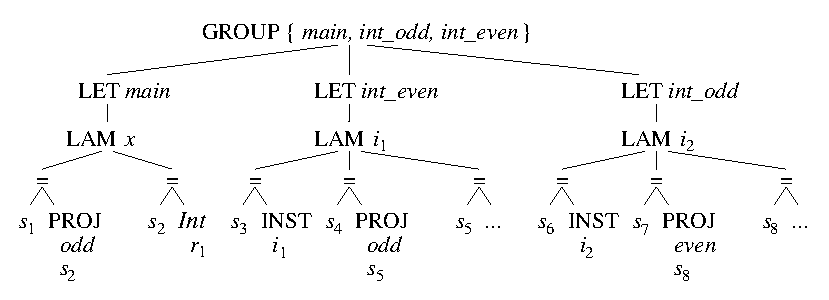
\includegraphics{3-Inference/fig/ordering/tree-start}
\end{center}

During type inference we perform a left to right, depth first traversal over the constraint tree. As we do this we delete constraints from the tree and add them to the type graph.  We start with a full tree and an empty type graph, and finish with a empty tree and a full graph. Internal nodes such as GROUP, LET and LAM organise the type constraints and represent the structure of the original program. We refer to the sub-tree headed by a GROUP, LET or LAM node as a GROUP, LET or LAM \emph{branch}. Once we have added all the constraints in a particular branch to the type graph we can delete the head-node as well. Deleting a LET node also triggers type generalisation, which we will discuss in a moment. Firstly, note that we when we arrive at an INST node, we can determine how the contained variable was bound by examining its parents. In the above example, we see that $i_1$ is lambda bound. In our practical implementation we maintain a stack of internal nodes for this purpose, pushing them onto the stack as we enter a branch, and popping as we leave.

As mentioned earlier, deletion of a LET node invokes generalisation of the type of the contained variable. However, recall from \S\ref{inference:generalisation} that before we generalise a type from the graph we must pack it into flat form, and this is only possible when the graph is in normal form. The graph is in normal form when no further reduction rules apply, and when it contains no unresolved PROJ or INST constraints. These two requirements ensure that we have solved all the constraints from a particular binding before we generalise its type. 

When performing type inference on a program whose bindings are not in dependency order, or whose bindings are mutually recursive, there will be situations when we wish to leave a LET branch but the graph is not in normal form. This will be because we have no type scheme to satisfy an INST node, or no type constructor to guide the reduction of a PROJ node. In these situations we remove the offending node from the graph and place it back in the tree, then restructure the tree so that further progress can be made before we need to perform the generalisation. This gives us time to infer the required type scheme, or determine the required type constructor, before we have to generalise the original type.

Both of these situations arise when typing the even/odd example on the previous page, so we will work through it now. We use $\bullet$ to indicate where we are in the traversal, and $\varepsilon$ to represent an empty branch. After descending into the right most branch and adding the $s_1$ and $s_2$ constraints we arrive at:

\begin{center}
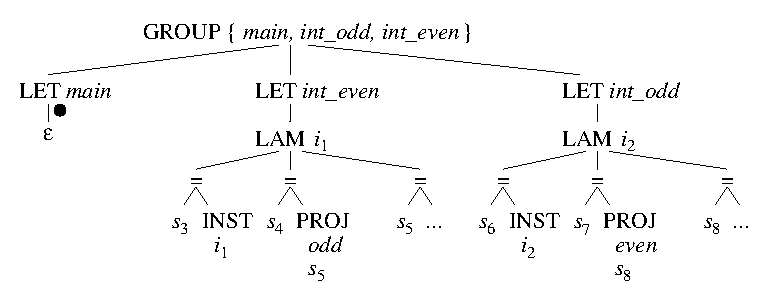
\includegraphics{3-Inference/fig/ordering/tree-main-gen}
\end{center}
\vspace{-2em}
The type graph is:
\begin{tabbing}
MMMMM	\= MM 	\= MM 		\= MMMMMM 	\= MM \kill
	\> *1	\> $\sim$	\> $s_1$	\> $= \ \rPROJ \ \iodd \ s_2$ \\
	\> *2	\> $\sim$	\> $s_2$	\> $= \ \iInt \ r_1$
\end{tabbing}
Now, we would like to leave the current branch and generalise the type of $\imain$, but before we do that we must reduce the graph to normal form. This requires that we resolve the projection constraint in *1. The projection constraint refers to $s_2$, which is constrained to be $\iInt \ r_1$. This means that we can look up the instance function to use from the corresponding dictionary. Here is the $\iInt$ dictionary again:

\code{
	\mc{4}{$\kproject \ \iInt :: \% \to * \ \kwith$} \\
	& $\ieven$	& $\sim \iintEven$	\\
	& $\iodd$	& $\sim \iintOdd$	\\
}

The $\iodd$ instance for integers is $\iintOdd$, so we can crush the $\rPROJ$ node in the graph into an $\rINST$ of this function's type. This yields:
\begin{tabbing}
MMMMM	\= MM 	\= MM 		\= MMMMMM 	\= MM \kill
	\> *1	\> $\sim$	\> $s_1$	\> $= \ \rINST \ \iintOdd$ \\
	\> *2	\> $\sim$	\> $s_2$	\> $= \ \iInt \ r_1$
\end{tabbing}

Now, we cannot actually instantiate the type for $\iintOdd$ yet because we haven't inferred it. Instead, we will defer further work on the type of $\imain$ and focus on $\iintOdd$ instead. We do this by removing the $s_1 = \ \rINST \ \iintOdd$ constraint from the graph and placing it back in the tree. We then move the LET $\iintOdd$ branch under LET $\imain$, so we can work on that before returning to generalise the type of $\imain$:
\begin{center}
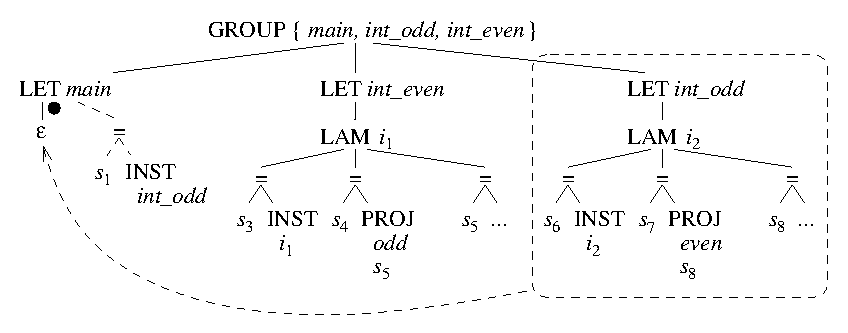
\includegraphics{3-Inference/fig/ordering/tree-main-gen-move}
\end{center}
Note that the $s_1 = \ \rINST \ \iintOdd$ constraint is placed \emph{after} the LET branch, so that the type for $\iintOdd$ will have been generalised before we need to instantiate it. Completing the move yields:
\begin{center}
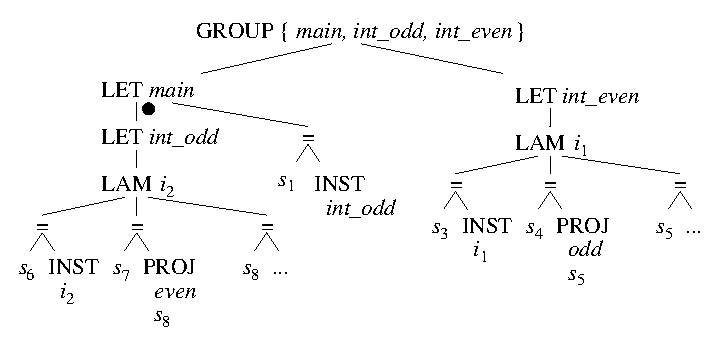
\includegraphics{3-Inference/fig/ordering/tree-main-gen-moved}
\end{center}

We can now continue our depth first traversal into the $\iintOdd$ branch, adding the constraints for $s_6$, $s_7$ and $s_8$ to the type graph. Assuming $s_8$ resolves to the type $\iInt \ r_2$, we end up with the following graph:
\begin{tabbing}
MMMMM	\= MM 	\= MM 		\= MMMMMM 	\= MM \kill
	\> *1	\> $\sim$	\> $s_1$	\> $= \ \bot$ \\
	\> *2	\> $\sim$	\> $s_2$	\> $= \ \iInt  \ r_1$ \\
	\> *3	\> $\sim$	\> $s_6$	\> $= \ s_{i_2}$ \\
	\> *4	\> $\sim$	\> $s_7$	\> $= \ \rPROJ \ \ieven \ s_8$ \\
	\> *5	\> $\sim$	\> $s_8$	\> $= \ \iInt \ r_2$
\end{tabbing}

Note that in our constraint tree, the constraint $s_6 = \rINST \ i_2$ appears under the $\rLAM \ i_2$ node, which tells us that $i_2$ is lambda bound. As we do not support higher rank types, lambda bound variables do not have polytypes. This means that we do not have to instantiate them, and we can simplify the $s_6$ constraint to $s_6 = s_{i_2}$. 

\clearpage{}
After the constraints from the $\iintOdd$ branch are added, our constraint tree is:
\begin{center}
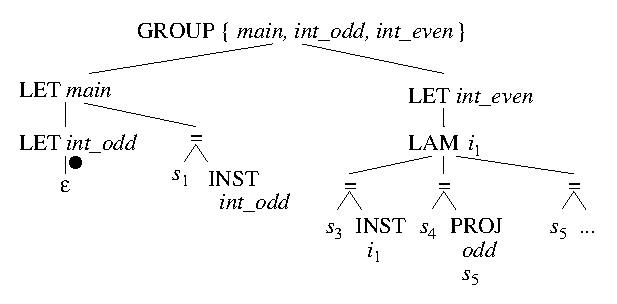
\includegraphics{3-Inference/fig/ordering/tree-intodd-gen}
\end{center}
\vspace{-2em}
And the graph is still:
\begin{tabbing}
MMMMM	\= MM 	\= MM 		\= MMMMMM 	\= MM \kill
	\> *1	\> $\sim$	\> $s_1$	\> $= \ \bot$ \\
	\> *2	\> $\sim$	\> $s_2$	\> $= \ \iInt  \ r_1$ \\
	\> *3	\> $\sim$	\> $s_6$	\> $= \ s_{i_2}$ \\
	\> *4	\> $\sim$	\> $s_7$	\> $= \ \rPROJ \ \ieven \ s_8$ \\
	\> *5	\> $\sim$	\> $s_8$	\> $= \ \iInt \ r_2$
\end{tabbing}

Now, the $\bullet$ shows that we are still inside the $\rLET \iintOdd$ branch. However, we cannot leave it yet and generalise the type of $\iintOdd$ because the graph contains an unresolved PROJ constraint, so is not in normal form. As before, this constraint refers to $s_8$ which an $\iInt$, so we can lookup the projection instance function from the corresponding dictionary and crush $\rPROJ \ \ieven \ s_8$ to $\rINST \ \iintEven$. Note that crushing a $\rPROJ$ constraint in this way corresponds to discovering part of the program's call tree, because we now know that $\iintOdd$ calls $\iintEven$. The new graph is:
\begin{tabbing}
MMMMM	\= MM 	\= MM 		\= MMMMMM 	\= MM \kill
	\> *1	\> $\sim$	\> $s_1$	\> $= \ \bot$ \\
	\> *2	\> $\sim$	\> $s_2$	\> $= \ \iInt  \ r_1$ \\
	\> *3	\> $\sim$	\> $s_6$	\> $= \ s_{i_2}$ \\
	\> *4	\> $\sim$	\> $s_7$	\> $= \ \rINST \ \iintEven$ \\
	\> *5	\> $\sim$	\> $s_8$	\> $= \ \iInt \ r_2$
\end{tabbing}
We still cannot generalise the type of $\iintOdd$ since it is not in normal form. As before, we will remove the offending $s_7 = \ \rINST \ \iintEven$ constraint from the graph and place it back in the tree, then reorganise the tree so we can make further progress. This gives:

\begin{center}
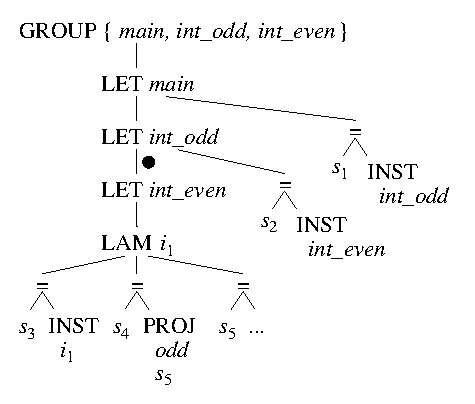
\includegraphics{3-Inference/fig/ordering/tree-intodd-gen-moved}
\end{center}

\clearpage{}
\begin{center}
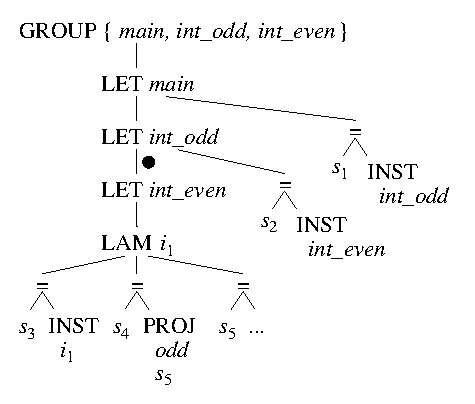
\includegraphics{3-Inference/fig/ordering/tree-intodd-gen-moved}
\end{center}
\vspace{-1em}
As before, we can continue our traversal by descending into the left of the tree, and adding the constraints for $s_3$, $s_4$ and $s_5$ to the graph. Once this is done we have:
\begin{center}
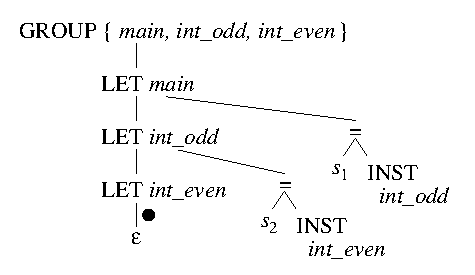
\includegraphics{3-Inference/fig/ordering/tree-inteven-gen}
\end{center}
After crushing the $s_4 = \rPROJ \ \iodd \ s_5$ constraint to $s_4 = \rINST \ \iintOdd$ the type graph becomes:
\begin{tabbing}
MMMMM	\= MM 	\= MM 		\= MMMMMM 	\= MM \kill
	\> *1	\> $\sim$	\> $s_1$	\> $= \ \bot$ \\
	\> *2	\> $\sim$	\> $s_2$	\> $= \ \iInt  \ r_1$ \\
	\> *3	\> $\sim$	\> $s_6$	\> $= \ s_{i_2}$ \\
	\> *4	\> $\sim$	\> $s_7$	\> $= \ \bot$ \\
	\> *5	\> $\sim$	\> $s_8$	\> $= \ \iInt \ r_8$ \\
	\> *6	\> $\sim$	\> $s_3$	\> $= \ s_{i_1}$ \\
	\> *7	\> $\sim$	\> $s_4$	\> $= \ \rINST \ \iintOdd$ \\
	\> *8	\> $\sim$	\> $s_5$	\> $= \ \iInt \ r_5$ 
\end{tabbing}
Note that at this point, we have discovered that $\iintOdd$ and $\iintEven$ are mutually recursive. This becomes clear when we place $s_4 = \ \rINST \ \iintOdd$ back in the tree:
\begin{center}
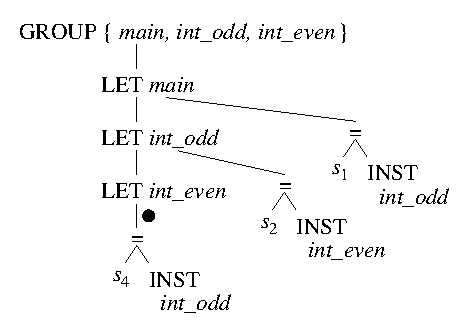
\includegraphics{3-Inference/fig/ordering/tree-inteven-moved}
\end{center}

\clearpage{}
In this tree, the fact that the $\rINST \ \iintOdd$ constraint appears under $\rLET \ \iintEven$ tells us that the binding for $\iintEven$ references $\iintOdd$, likewise, $\iintOdd$ references $\iintEven$. As with Haskell \cite{jones:typing-haskell}, in the absence of polymorphic recursion we type mutually recursive bindings using monotypes for the bound variables. This allows us to rewrite the $s_4 = \rINST \ \iintOdd$ and $s_2 = \rINST \ \iintEven$ constraints to $s_4 = s_{\iintOdd}$ and $s_2 = s_{\iintEven}$. These can be added directly to the graph without needing to instantiate type schemes for $\iintOdd$ or $\iintEven$. Note that in this example we have elided the majority of the constraints from the program. In practice, after adding the two constraints $s_4 = s_{\iintOdd}$ and $s_2 = s_{\iintEven}$ we will need to perform unifications and other reductions to return it to normal form. 

Finally, when leaving the $\rLET \ \iintEven$ and $\rLET \ \iintOdd$ branches, we must wait until we are outside all the branches of a binding group before we generalise their types. This ensures that all constraints from all bindings in the group have been processed, and that we treat the group as a single unit. 



\subsection{Comparison with Helium. 2002 -- \\
 Heeren, Hage, Swierstra.}
There are many degrees of freedom to the order in which constraints are processed. If a program contains multiple type errors, then solving constraints in a different order affects which errors are encountered first. For all other programs, changing the order should not affect the substance of the solution.

However, there \emph{is} one overriding restriction. Before the type of a let-bound variable can be generalised into a type scheme, all the constraints from the right of the binding must have been added to the graph. If we fail to do this then the resulting scheme may be instantiated at several different types before we encounter a constraint that would have prevented part of it from being generalised. 

We handle this restriction by expressing the type constraints as a tree. Each let-binding corresponds to a branch in the tree, and during our traversal we use the structure of the tree to ensure that constraints from sub-branches are added to the graph before the type of the binding is generalised. In contrast, in the Helium~\cite{heeren:constraint-type-inferencing, heeren:generalising-hm} compiler, the type constraints fed to the solver have a flat structure, and the requirement to process constraints from the right of a let-binding before generalising the type of the bound variable is handled in a different way.

Helium uses a constraint of the following form: 

\code{
	$\tau_1 \leq_M \tau_2$
}

This constraint says that $\tau_1$ is obtained by first generalising $\tau_2$ with respect to the set of monomorphic variables $M$, and then instantiating the resulting type scheme. The restriction is enforced by requiring that all constraints involving type variables that are present in $\tau_2$, but cannot appear in $M$, are processed first. This requirement ensures that the form of $\tau_2$ cannot change once we make the type scheme. We feel that this is a more elegant solution than our own method of dynamically reordering constraint trees. 

On the other hand we are unsure whether it is possible to adapt Helium's algorithm to deal with the mutually recursive projection definitions considered in this section. In \cite{heeren:constraint-type-inferencing}, the rules given to extract type constraints from the source program require the calculation of the binding dependency graph, and we have seen that this is not possible with recursive projections. It would seem that to calculate the binding dependency graph on the fly, we must retain information about which projections appear in which bindings. It may well be possible to construct a hybrid of Helium's system and our own, but we have not looked into it in detail.

We also wonder about the run time cost of determining which of the $\tau_1 \leq_M \tau_2$ constraints in the graph are ready to be processed. Using a flat constraint tree provides more freedom to choose the order in which constraints are considered, but using a hierarchical one provides more direction. Chapter 4 of \cite{heeren:top-quality-error-messages} contains further discussion of the pros and cons of several related approaches.

Besides the restriction outlined above, it is also important that enough type information makes it into the graph before we are forced to resolve projection constraints. In our current implementation, a particular type is only generalised the first time we need to instantiate it. If there are no bound occurrences of a variable in the module being compiled, which is common for library code, then its type is generalised after all other information is added to the graph. We are unsure whether our chosen approach admits edge cases where a particular projection constraint ``should have'' been resolved, but wasn't. This would create spurious ambiguous projection errors, but we have not noticed any so far.




 





\clearpage{}
\section{Type Classes}
\label{inference:type-classes}

It is straightforward to add basic support for type class constraints to a graph based inference algorithm. This includes support for ``baked in'' constraints such as $\iMutable$ and $\iPure$, as well as programmer defined constraints such as $\iShow$ and $\iEq$. 

The additions to the language are:

% -- Declarations
\vspace{-1em}
\subsubsection{Declarations}
\vspace{-1ex}
\begin{tabbing}
	MM 	\= MM \= MMMMMMMMMMMMMMMMMM \= MMMMMMM \kill
	$\idecl$ \> $\to$ 	\> $\dots$ \\
		\> \ $\mid$	\> $\kclass \ C \ \ov{a} \ \kwhere \ \ov{x :: \varphi}$  
				\> (type class declaration) \\[0.5ex]
		\> \ $\mid$	\> $\kinstance \ C \ \ov{\tau} \ \kwhere \ \ov{x = t}$  
				\> (type class instance)
\end{tabbing}

% -- Types 
\vspace{-2em}
\subsubsection{Types}
\vspace{-1ex}
\begin{tabbing}
	MM 	\= MM \= MMMMMMM \= MMMMMMMMMMM \= MMMM \kill
	$\varphi$, $\tau$, $\sigma$, $\varsigma$	\\
		\> \ $\to$	\> \dots \\
		\>  \ $\mid$	\> $\iReadT \ \tau$	\> $\mid \ \iWriteT \ \tau$	
				\> (effect constructors)
\end{tabbing}


% -- Constraints
\vspace{-2em}
\subsubsection{Constraints}
\vspace{-1ex}
\begin{tabbing}
	MM 	\= MM \= MMMMMMM \= MMMMMMMMMMM \= MMMM \kill
	$\chi$ 	\> $\to$	\> \dots 
		\\[0.5ex]
		\> \ $\mid$	\> $C \ \ov{\tau}$ 
				\> \> (value type classes)
		\\[0.5ex]
		\> \ $\mid$	\> $\iShape \ \tau \ \tau'$ 
						\> $\mid \ \iLazyH \ \tau$ 
				\> 
		\\[0.5ex]
		\> \ $\mid$	\> $\iConstT \ \tau$	\> $\mid \ \iMutableT \ \tau$
				\> 
		\\[0.5ex]
		\> \ $\mid$	\> $\iConst \ r$ 	\> $\mid \ \iMutable \ r$	
				\> (region classes)	
		\\
		\> \ $\mid$	\> $\iLazy \ r$		\> $\mid \ \iDirect \ r$  
				\> 
		\\[0.5ex]
		\> \ $\mid$	\> $\iPure \ \sigma$	\>				
				\> (effect class)	
		\\[0.5ex]
		\> \ $\mid$	\> $\iEmpty \ \varsigma$ \>				
				\> (closure class)	
\end{tabbing}

The new declarations behave the same way as their Haskell counterparts. We use $C$ to represent the programmer defined type class constructors such as $\iShow$ and $\iEq$. The meanings of $\iShape$, $\iConstT$ and $\iMutableT$ are discussed in \S\ref{System:TypeClassing}. The meanings of $\iLazy$, $\iLazyH$ and $\iDirect$ were discussed in \S\ref{System:Effects:lazy-and-direct}. $\iPure$ is discussed in \S\ref{System:Effects:purification} and $\iEmpty$ is discussed in \S\ref{System:Closure:empty}.

When performing inference we represent type class constraints as extra nodes in the graph. For example, the type:

\code{
	$s_{\iupdateInt}$ 
		& $= \iInt r_1 \to \iInt r_2 \lfuna{e_1 \ c_1} ()$ \\
		& $\rhd \ e_1 \tme \iRead r_2 \lor \iWrite r_1$ \\
		& $, \  \ c_1 \tme x : r_1$ \\
		& $, \ \ \iMutable \ r_1$ 	
}

Would be represented as:
\begin{tabbing}
MMMMM	\= MM 	\= MM 		\= MMMMMM 	\= MM \kill
	\> *1	\> $\sim$	\> $s_{\iupdateInt}$	
					\> $= \ \iInt \ r_1 \to \iInt \ r_2 \lfuna{e_1 \ c_1} ()$ \\
	\> \ !1	\> $\sim$	\> $e_1$	\> $\tme \ \iRead \ r_2 \lor \iWrite \ r_1$ \\
	\> \$1	\> $\sim$	\> $c_1$	\> $\tme \ x : r_1$ \\
	\> $\Diamond1$	\> $\sim$	\> $\iMutable \ r_1$ 
\end{tabbing}

In the type graph we use $\Diamond$ as an identifier for type class equivalence classes.\footnote{Perhaps the type theorist union should start a petition to introduce more synonyms for ``constraint'', and ``class.''} Note that in $\Diamond1$ we have not used an = or $\tme$ operator. Both of these operators are binary and infix, but $\iMutable$ is unary and prefix. We store multi-parameter type class constraints such as $\iShape$ in the same way.

Following on from the section on generalisation \S\ref{inference:generalisation}, when we trace a type from the graph we must also include any type class constraints that reference variables in the body of the type. For example, if we were to re-trace the type of $\iupdateInt$ from the graph, we would need to include $\iMutable \ r_1$. In a real implementation it would be a disaster if we had to inspect every equivalence class in the graph to find all the appropriate constraints. In DDC we mitigate this problem associating each value, region, effect and closure equivalence class, with a set of type class equivalence classes that contain references to it.

Although the programmer defined type classes do not have super class constraints, there are implicit super class constraints on some of the built in ones. We need to reduce these constraints when performing type inference, and the rest of this section discusses how this is done.


%--
\subsection{Deep Read/Write}

\begin{tabbing}
	M \= MMMMMMMMM \= MMMMMMMM \= MMMMM \kill
	\> (deep read data)	\> $\{ \ s = T_{\kappa} \ \ov{a}$, 
				\> $e \tme \iReadT \ s \ \}$ 
	\\
	\> \qq \qq $\vvdash$	\> $\{ \ s = T_{\kappa} \ \ov{a}$, 
				\> $e \tme \ov{\iReadT \ b} \lor \ov{\iRead \ r} \}$ 
	\\[1ex]
	\> \qq \qq	
		\begin{tabular}{lllll}
		where 	& $\ov{b} \in \{ \ b'$	
					& $| \ b'  \gets \ov{a},$
					& $b' :: *,$
					& $b' \in \imv(\emptyset, \ T_{\kappa} \ \ov{a}) \ \}$ \\
			& $\ov{r}    \in \{ \  r'$	
					& $| \ r'   \gets \ov{a},$
					& $r' :: \%,$ 
					& $r' \in \imv(\emptyset, \ T_{\kappa} \ \ov{a}) \ \}$ 
		\end{tabular}
\end{tabbing}

A deep read effect such as $\iReadT \ a$ represents a read on any region variable contained within the as-yet unknown type $a$. The $\iReadT$ constructor has kind $* \to \ !$, and the ``T'' in $\iReadT$ stands for ``value type''. This distinguishes it from the standard $\iRead$ constructor that works on single regions.

When reducing a deep read on a data type $T \ \ov{\varphi}$, we first separate the argument variables $a$ according to their kinds. Reads on region variables are expressed with the $\iRead$ constructor, and reads on value type variables are be expressed with $\iReadT$. Reads on effect and closure arguments can be safely discarded, as there is no associated action at runtime.

It is only meaningful to read (or write) material variables, hence the clauses \mbox{$b' \in \imv(\emptyset, \ T_{\kappa} \ \ov{a})$} and \mbox{$r' \in \imv(\emptyset, \ T_{\kappa} \ \ov{a})$}. In these clauses, it is safe to use $\emptyset$ for the constraint set. As mentioned in \S\ref{inference:material-regions}, the $\imv$ function expresses a simple reachability analysis, but so does the (deep read data) reduction rule. The appropriate read effects will be generated when we perform further reductions on the resulting graph.

Deep writes are handled similarly to deep reads. Note that an implementation must be careful about applying these reduction rules when there are loops through the value portion of the type graph. For example, if we had the following constraints:

\code{
	$\{ \ s = \iList \ r \ s, \ e \tme \iReadT s \ \}$
}

This graph cannot be reduced to normal form because each application of (deep read data) to $\iReadT s$ generates $\iRead r$ as well as another $\iReadT s$ effect.

\begin{tabbing}
	M \= MMMMMMMMM \= MMMMMMMM \= MMMMM \kill
	\> \ \ (deep read fun)	\> $\{ \ s = \tau_1 \lfuna{\sigma \ \varsigma} \tau_2$, 
				\> $e \tme \iReadT \ s \ \}$ 
	\\
	\> \qq \qq $\vvdash$	\> $\{ \ s = \tau_1 \lfuna{\sigma \ \varsigma} \tau_2$, 
				\> $e \tme \bot \ \}$ 
\end{tabbing}

The rule (deep read fun) shows that deep reads (and writes) on function types can be removed from the graph. Function values do not contain material objects that are capable of being updated.


%--
\subsection{Deep Mutable/Const}

Deep mutability and constancy constraints are reduced in a similar way to deep read and write effects.

\begin{tabbing}
	M \= MMMMMMMMM \= MMMMMMMM \= MMMMM \kill
	\> \ \ \ (deep mutable)	\> $\{ \ s = T \ \ov{a}$, 
				\> $\iMutableT \ s \ \}$ 
	\\
	\> \qq \qq $\vvdash$	\> $\{ \ s = T \ \ov{a}$, 
				\> $\ov{\iMutableT \ b}, \ \ov{\iMutable \ r} \ \}$ 
	\\[1ex]
	\>  \qq \qq	
		\begin{tabular}{lllll}
		where 	& $\ov{b} \in \{ \ b'$	
					& $| \ b'  \gets \ov{a},$
					& $b' :: *,$
					& $b' \in \imv(\emptyset, \ T_{\kappa} \ \ov{a}) \ \}$ \\
			& $\ov{r}    \in \{ \  r'$	
					& $| \ r'   \gets \ov{a},$
					& $r' :: \%,$ 
					& $r' \in \imv(\emptyset, \ T_{\kappa} \ \ov{a}) \ \}$ 
		\end{tabular}
\end{tabbing}


%--
\subsection{Purification}

\begin{tabbing}
	MMM \= MMMMMMM \= MMMMMMMM \= MMMMM \= MMMMM \kill
	\> \ \ (purify)	\> $\{ \ e \tme \iRead \ r$, 
			\> $\iPure \ e \ \}$ 
	\\
	\> \qq $\vvdash$	
			\> $\{ \ e \tme \iRead \ r$, 
			\> $\iPure \ e$,
			\> $\iConst \ r \}$ 
\end{tabbing}

\begin{tabbing}
	MMM \= MMMMMMM \= MMMMMMMM \= MMMMM \= MMMMM \kill
	\> (deep purify)	
			\> $\{ \ e \tme \iReadT \ s$, 
			\> $\iPure \ e \ \}$ 
	\\
	\> \qq $\vvdash$	
			\> $\{ \ e \tme \iReadT \ s$, 
			\> $\iPure \ e$,
			\> $\iConstT \ s \}$ 
\end{tabbing}

\begin{tabbing}
	MMM \= MMMMMMM \= MMMMMMMM \= MMMMM \= MMMMM \kill
	\> (purify trans)	
			\> $\{ \ e_1 \tme e_2$, 
			\> $\iPure \ e_1 \ \}$ 
	\\
	\> \qq $\vvdash$	
			\> $\{ \ e_1 \tme e_2$, 
			\> $\iPure \ e_1$,
			\> $\iPure \ e_2 \}$ 
\end{tabbing}


To purify a $\iRead$ effect on a region $r$, we constrain that region to be constant by adding $\iConst \ r$ to the graph. Purification of deep reads is similar. As discussed in \S\ref{System:Effects:purification-higher-order}, we choose to leave the original $\iRead$ effect in the graph, though we could equally remove it.

We must leave the $\iPure \ e$ constraint in the graph. If the equivalence class containing $e$ is unified with another, then these new effects need to be purified as well. 

For example, suppose we had the following constraint set:

\qq (1) \quad
\begin{tabular}{llllll}
	$\{$
	& $s = a \lfuna{e_1} b$,	& $e_1 \tme \iRead \ r_1$, 	& $\iPure \ e_1$, \\
	& $s = a \lfuna{e_2} b$, 	& $e_2 \tme \iRead \ r_2$, 	& $\iMutable \ r_2$
	& $\}$
\end{tabular}
\bigskip

If we were to set $r_1$ constant while removing the $\iPure \ e_1$ constraint we would get:

\qq (2) \quad
\begin{tabular}{llllll}
	$\{$
	& $s = a \lfuna{e_1} b$, 	& $e_1 \tme \iRead \ r_1$,	& \\
	& $s = a \lfuna{e_2} b$, 	& $e_2 \tme \iRead \ r_2$, 	& $\iMutable \ r_2$, \\
	& $\iConst \ r_1$ 		&				&	
	& $\}$ \qq	(bad purify, 1)
\end{tabular}
\bigskip

\clearpage{}
Performing unification on $s$ gives:

\qq (3) \quad
\begin{tabular}{llllll}
	$\{$
	& $s \ = a \lfuna{e_1} b$,	& $e_1 \tme \iRead \ r_1$,	& \\
	& 	 			& $e_1 \tme \iRead \ r_2$,	& $\iMutable \ r_2$, \\
	& $\iConst \ r_1$, 		& $e_1 = e_2$			&	
	& $\}$ \qq	(unify fun, 2)
\end{tabular}
\bigskip

Now, although we used to have a purity constraint on $e_1$, this effect now includes a read of the mutable region $r_2$. In addition, there is nothing left in the constraint set to indicate that such an effect is in any way invalid. On the other hand, if we were to take our original constraint set and perform the unification first, then we would get:

\qq (4) \quad
\begin{tabular}{llllll}
	$\{$
	& $s \ = a \lfuna{e_1} b$,	& $e_1 \tme \iRead \ r_1$, 	& $\iPure \ e_1$, \\
	& 	 			& $e_1 \tme \iRead \ r_2$, 	& $\iMutable \ r_2$, \\
	& $e_1 = e_2$ 			& 			&	
	& $\}$ \qq (unify fun, 1)
\end{tabular}
\bigskip

Applying the bad purify rule to this new set yields:

\qq (5) \quad
\begin{tabular}{llllll}
	$\{$
	& $s \ = a \lfuna{e_1} b$,	& $e_1 \tme \iRead \ r_1$, 	& \\
	& 	 			& $e_1 \tme \iRead \ r_2$, 	& $\iMutable \ r_2$, \\
	& $e_1 = e_2$,			& $\iConst \ r_1$,		& $\iConst \ r_2$ 
	& $\}$ \qq (bad purify, 4)
\end{tabular}
\bigskip

In this case we have both $\iMutable \ r_2$ and $\iConst \ r_2$ in the final constraint set, which indicates a type error. Removing the purity constraint from the graph has caused our reduction to be non-confluent. 


% -----------------------------------------------------------------------------
\subsection{Shape}

\begin{tabbing}
	MMM \= MMMMMMM \= MMMMMMMM \= MMMMM \= MMMMM \kill
	\> (shape left)	\> $\{ \ s_1 = T_{\kappa} \ \ov{a}$, 
			\> $\iShape \ s_1 \ s_2 \ \}$
	\\[1ex]
	\> \qq $\vvdash$
			\> $\{ \ s_1 = T_{\kappa} \ \ov{a}$,
			\> $s_2 = \varphi' \ \} \ \cup \ 
				\iaddShape (\emptyset, \ T_{\kappa} \ \ov{a}, \ \varphi') $ 
	\\[1ex]
	\> 		\> where \ $\varphi' = \ifreshen(\emptyset, \ T_{\kappa} \ \ov{a})$
\end{tabbing}

\begin{tabbing}
	MMM \= MMMMMMM \= MMMMMMMM \= MMMMM \= MMMMM \kill
	\> (shape right) \> $\{ \ s_2 = T_{\kappa} \ \ov{a}$, 
			 \> $\iShape \ s_1 \ s_2 \ \}$
	\\[1ex]
	\> \qq $\vvdash$
			\> $\{ \ s_2 = T_{\kappa} \ \ov{a}$,
			\> $s_1 = \varphi' \ \} \ \cup \ 
				\iaddShape (\emptyset, \ T_{\kappa} \ \ov{a}, \ \varphi')$ 
	\\[1ex]
	\> 		\> where \ $\varphi' = \ifreshen(\emptyset, \ T_{\kappa} \ \ov{a})$
\end{tabbing}

\quad
\begin{tabular}{llllll}
	\mc{2}{$\ifreshen(\iSM, \ a_\kappa)$} \\
	& $| \ a_{\kappa} \in \iSM \ \trm{and} \ \kappa \in \{ *, \% \}$
	& $ = a_\kappa' \ \trm{fresh}$
	\\[1ex]
	\mc{2}{$\ifreshen(\iSM, \ T_{\kappa} \ \ov{\varphi})$}
		& $ = T_{\kappa} \ \ \ov{\ifreshen(\iSM \cup \ismv(\emptyset, T_{\kappa} \ \ov{\varphi}), \ \varphi)}$ 
	\\[1ex]
	\mc{2}{$\ifreshen(\iSM, \ \varphi)$}	
		& $ = \varphi$
	\\[2em]
	%
\end{tabular}

\quad
\begin{tabular}{llllll}
	%
	\mc{2}{$\iaddShape(\iSM, \ a_{*}, \ a_{*}')$} \\
	& $| \ a_{*} \in \iSM \ \trm{and} \ a_{*} \neq a_{*}'$
	& $ = \{ \ \iShapeTwo a_* \ a_*' \ \}$
	\\[1ex]
	\mc{2}{$\iaddShape(\iSM, \ T_{\kappa} \ \ov{\varphi}, \ T_{\kappa} \ \ov{\varphi'})$}
		& $ = \bigcup \ov{\iaddShape(\iSM \cup \ismv(\emptyset, T_{\kappa} \ \ov{\varphi}), \ \varphi, \ \varphi')}$
	\\[1ex]
	\mc{2}{$\iaddShape(\iSM, \ \varphi, \ \varphi')$}
		& $ = \emptyset$
\end{tabular}

\bigskip
When reducing a constraint like $\iShape \ s_1 \ s_2$, the choice of what rule to use depends on whether we have a type constructor for $s_1$ or $s_2$. If we have a constructor for $s_1$, we can use this as a template to constrain the type of $s_2$, and \emph{vice versa}. If we have a constructor for both $s_1$ and $s_2$, then it does not matter which of the rules we use. 

\subsubsection{Example}
We will use the $\iFunThing$ type as an example. A $\iFunThing$ can contain an integer, a character, a function that takes an integer, or a thing of arbitrary type.

\code{
	\mc{3}{$\kdata \ \iFunThing \ r_1 \ r_2 \ a_1 \ a_2 \ e_1 \ c_1$} \\
		& $=$	& $\iFInt \  (\iInt \ r_1)$ \\
		& \ $|$ & $\iFChar \ (\iChar \ r_2)$ \\
		& \ $|$	& $\iFFun \ (\iInt \ r_2 \lfuna{e_1 \ c_1} a_1)$ \\
		& \ $|$	& $\iFThing \ a_2$
}

% The kind of $\iFunThing$ is $\% \to \% \to * \to * \to \: ! \to \$ \to *$. 

Suppose we have constraints: 

\quad\quad\quad
\begin{tabular}{llllll}
	$\{$
	& $s_1 \ = \iFunThing \ r_1 \ r_2 \ s_2 \ s_3 \ e_1 \ c_1$ \\
	& $s_2 \ = \iInt \ r_3$ \\
	& $s_3 \ = \iInt \ r_4$ \\
	& $e_1 \ \tme \iRead \ r_2 \lor \iRead \ r_5$ \\
	& $c_1 \ \tme \iInt \ r_5$ \\
	& $\iShape \ s_1 \ s_1'$ 
	& $\}$
\end{tabular}
\bigskip

As we have a constructor for $s_1$ we can use the (shape left) rule. The material variables of $\iFunThing \ r_1 \ r_2 \ s_2 \ s_3 \ e_1 \ c_1$ are:

\code{
	$\imv(\emptyset, \iFunThing \ r_1 \ r_2 \ s_2 \ s_3 \ e_1 \ c_1)$ & $= \{ r_1, \ r_2, \ a_2 \}$
}

Whereas the immaterial variables are:

\code{
	\: $\iiv(\emptyset, \iFunThing \ r_1 \ r_2 \ s_2 \ s_3 \ e_1 \ c_1)$ & $= \{ r_2, \ e_1, \ c_1, a_1 \}$
}

This means the strongly material variables are:

\code{
	$\ismv(\emptyset, \iFunThing \ r_1 \ r_2 \ s_2 \ s_3 \ e_1 \ c_1)$ & $= \{ r_1, \ a_2 \}$
}

Note that when reducing the $\iShape$ constraint, region variables that are only reachable from the closure of a type, such as $r_5$, are not counted as material. Similarly to the example given in \S\ref{System:TypeClassing:shape-immaterial}, the programmer cannot copy objects in such regions, so we do not freshen the associated region variables. This is achieved in part by passing $\emptyset$ as the first argument of $\ifreshen$ and $\iaddShape$, instead of the full set of constraints being reduced. This ensures that these functions do not have information about the $c_1$ constraint. 

The alternative would be to freshen $c_1$ as well, and create a new constraint $c_1' \tme \iInt \ r_5'$. We would also need to create a new version of the constraint on $e_1$, and ensure that this referred to the copied closure. Of course, actually copying the objects in the closures of functions would require additional support from the runtime system, so we have not considered it further.

Applying the $\ifreshen$ function to the type of $s_1$ gives us the new type:

\code{
	$s_1' = \iFunThing \ r_1' \ r_2 \ s_2 \ s_3' \ e_1 \ c_1$ \qq with $r_1', s_3'$ fresh
}

\clearpage{}
Applying the $\iaddShape$ function provides $\iShape$ constraints on the components of this type:

\code{
	 \mc{4}{$\iaddShape (\emptyset	
				, \ \iFunThing \ r_1 \ r_2 \ s_2 \ s_3 \ e_1 \ c_1
				, \ \iFunThing \ r_1' \ r_2 \ s_2 \ s_3' \ e_1 \ c_1)$} 
		\\[1em]
   		& $\equiv$	& $\iaddShape(\iSM, \ r_1, \ r_1')$ & $\cup \ \iaddShape(\iSM, \ r_2, \ r_2)$ \\
		& $\cup$	& $\iaddShape(\iSM, \ s_2, \ s_2)$  & $\cup \ \iaddShape(\iSM, \ s_3, \ s_3')$ \\
		& $\cup$	& $\iaddShape(\iSM, \ e_1, \ e_1)$  & $\cup \ \iaddShape(\iSM, \ c_1, \ c_1)$ \\
		&		& $\kwhere \ \iSM = \{ r_1, \ s_3 \}$
		\\[1ex]
		& $\equiv$	& $\iShape \ s_3 \ s_3'$
}

So our final result is:

\quad\quad\quad
\begin{tabular}{llllll}
	$\{$
	& $s_1 \ = \iFunThing \ r_1 \ r_2 \ s_2 \ s_3 \ e_1 \ c_1$ \\
	& $s_2 \ = \iInt \ r_3$ \\
	& $s_3 \ = \iInt \ r_4$ \\
	& $e_1 \ \tme \iRead \ r_2 \lor \iRead \ r_5$ \\
	& $c_1 \ \tme \iInt \ r_5$ \\[1ex]
	& $s_1' = \iFunThing \ r_1' \ r_2 \ s_2 \ s_3' \ e_1 \ c_1$ \\
	& $\iShape \ s_3 \ s_3'$
	& $\}$
\end{tabular}

Note that in the new type $\iFunThing \ r_1' \ r_2 \ s_2 \ s_3' \ e_1 \ c_1$, the fresh variables $r_1'$ and $s_3'$, correspond to just the components of the underlying $\iFunThing$ values that can potentially be coppied. $r_2$ and $s_2$ are not freshened because these variables are used in the parameter and return types of an embedded function value. Likewise $e_1$ and $c_1$ are not freshened because they do not represent data objects.



\section{Error Reporting}
\label{inference:errors}
In a constraint based inference algorithm, the natural way to include error reporting is to add justifications to each of the constraints extracted from the source program. These justifications can be maintained as the graph is reduced, and if we encounter an error we can use the justification to determine why the conflicting constraints were added to the graph. This approach is outlined by Wand \cite{wand:finding-type-errors}, and elaborated by Duggan \cite{duggan:explaining-type-inference}, Stuckey \cite{stuckey:improving-type-error-diagnosis} and Heeren \cite{heeren:top-quality-error-messages}. We will give an overview of the general ideas, and focus on how we manage the constraints that are specific to Disciple.

Consider the $\isuccDelay$ program from \S\ref{System:Effects:purification}

\code{
	\mc{2}{$\isuccDelay \ ()$} \\
 	$ \ = \ \kdo$	& $x = 5$ \\
               		& $y = \isucc \ @ \ x$ \\
			& $\dots$ \\ 
			& $x := 23$ \\
			& $\dots$
}

This program has a purity conflict. The binding for $y$ creates a suspension that will read the value of $x$, but later in the program this value is updated. This implies that the value of $y$ will depend on when it is forced, which is a program behaviour we take as being invalid. Here are the syntax trees for the three statements in the do-block, after desugaring:

\begin{center}
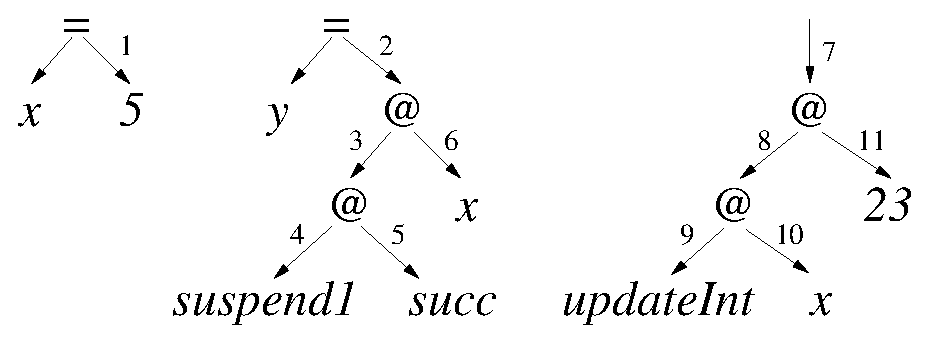
\includegraphics[scale=0.5]{3-Inference/fig/errors/suspend-succ.eps}
\end{center}

After extracting type constraints and solving them, we are left with a type graph containing the following equivalence classes:

\vspace{-1ex}
\begin{tabbing}
MMMMM	\= MM 	\= MM 		\= MMMMMMMMMM 		\= MM \kill
	\> *1	\> $\sim$	\> $s_x, \ a, \ s_1 \ s_6, \ s_{10}$		
				\> $= \ \iInt \ r_1$ 
	\\
	\> *2	\> $\sim$	\> $s_y, \ b, \ s_2$	
				\> $= \ \iInt  \ r_6$ 
	\\
	\> *3	\> $\sim$	\> $s_3$		
				\> $= \ s_x \lfuna{e_2 \ c_2} \ s_y$ 
	\\
	\> *4	\> $\sim$	\> $s_4$
				\> $= \ s_5 \lfuna{e_3 \ c_3} s_3$ 
	\\
	\> *5	\> $\sim$	\> $s_5$
				\> $= \ s_x \lfuna{e_5 \ c_5} s_y$\\
	\> \qq \dots \\
	\> \ !1	\> $\sim$	\> $e_5, \ e_6$
				\> $\tme \ \iRead \ r_1$ 
	\\
	\> \ !2 \> $\sim$	\> $e_7, \ e_9$
				\> $\tme \ \iRead \ r_{10} \lor \iRead \ r_1$
	\\
	\> \qq \dots \\
	\> \ $\Diamond$1 \> $\sim$ \> $\iPure \ e_5$ \\
	\> \ $\Diamond$2 \> $\sim$ \> $\iConst \ r_1$ \\
	\> \ $\Diamond$3 \> $\sim$ \> $\iMutable \ r_1$
\end{tabbing}

This graph contains an obvious type error. $\Diamond$2 contains a constraint that requires $r_1$ to be constant, while $\Diamond$3 contains a constraint that requires it to be mutable. As discussed in \S\ref{Core:Witnesses}, we cannot convert this example to a valid core program because there is no way to construct witnesses for both of these constraints at once. Unfortunately, the \emph{reason} for this error is not so obvious. It would be unhelpful for a compiler to simply report that it ``cannot create core witnesses'', or that ``$\iConst \ r_1$ conflicts with $\iMutable \ r_1$''. Neither of these messages help us determine what part of the program caused the error, or suggest how we might resolve it.

\subsection{Constraint justifications}

As mentioned previously, we track the source of type errors by attaching justifications to each of the constraints from the program. For example:

\begin{tabbing}
MMMMM	\= MMMM 		\= MMMMMMMMMMM 		\= MMMMMMMMM		\= MM \kill
	\> $s_{4u}$	\> $= s_5 \lfuna{e_3 \ c_3} s_3$		\> $| \ i_1$ 
	\\[0.5ex]
	\> $s_{4d}$ 	\> $= \rINST \ s_{\isuspend}$ 			\> $| \ i_2$
	\\[0.5ex]
	\> $s_{4u}$	\> $= s_{4d}$					\> $| \ i_3$
	\\[0.5ex]
	\> $s_5$	\> $= \rINST \ s_{\isucc}$			\> $| \ i_4$
	\\[0.5ex]
	\> $s_9$	\> $= \rINST \ s_{\iupdateInt}$			\> $| \ i_5$
	\\[0.5ex]
	\> $i_1$	\> $= \iIApp \ 3 \ \isuspend \ \isucc$ 
	\\
	\> $i_2$	\> $= \iIVar \ 3 \ \isuspend$
	\\
	\> $i_3$	\> $= \iIUseDef 3 \ \emptyset$
	\\
	\> $i_4$	\> $= \iIVar \ 3 \ \isucc$
	\\
	\> $i_5$	\> $= \iIVar \ 5 \ \iupdateInt$
	\\
	\> \dots
\end{tabbing}

We now write value type constraints as $s = \tau \ | \ i$, where $s$ is a type variable, $\tau$ is a type, and $i$ is a \emph{source information variable}. In this presentation we will refer to source information as just ``information''. We extend region, effect, closure and type class constraints in a similar way. Information variables are bound to information expressions in separate constraints. Information expressions are built with \emph{information constructors} such as $\iIApp$ and $\iIVar$. 

We give information constructors informal, descriptive kinds:

\code{
	$\iIApp$ 	&	$:: \trm{num} \to \trm{exp} \to \trm{exp} \to \trm{info}$ \\
	$\iIVar$ 	&	$:: \trm{num} \to \trm{var} \to \trm{info}$ \\
	$\iIUseDef$ 	&	$:: \trm{num} \to \trm{Set info} \to \trm{info}$
}

$\iIApp$ takes a line number and two expressions. It produces information that says a particular constraint is due to the application of these two expressions, on that line of the source program. $\iIVar$ produces information that says a constraint is due to the use of a particular variable. $\iIUseDef$ produces information that says a constraint is due to the fact that the definition of a variable must match its use. The first argument of $\iIUseDef$ is a line number as before, but the second argument is a set of other information expressions. We will see how this works in a moment. 

We now discuss how to record source information in the type graph representation. For constraints involving a constructor, we can take the information variable from the constraint, and use it to annotate the constructor as it is placed into an equivalence class. When performing an instantiation due to an $\rINST$ constraint, the information variable on the $\rINST$ constructor is propagated to all the new constructors created during the instantiation. For example, after adding the above constraints to the type graph and performing the instantiations we get:

\begin{tabbing}
MMMMM	\= MM 	\= MM 		\= MMMMMMMMMM 		\= MM \kill
	\> *1	\> $\sim$	\> $s_{4u}$		
				\> $= \ (s_5 \lfuna{e_3 \ c_3} s_3)^{i_1}$
	\\
	\> *2	\> $\sim$	\> $s_{4d}$
				\> $= \ (s_{41} \lfuna{e_{4d} \ c_{4d}} s_{42})^{i_2}$ 
	\\
	\> *3	\> $\sim$	\> $s_{41}$		
				\> $= \ (a \lfuna{e_{41} \ c_{41}} \ b)^{i_2}$ 
	\\
	\> *4	\> $\sim$	\> $s_{42}$
				\> $= \ (a \lfuna{e_{42} \ c_{42}} \ b)^{i_2}$ 
	\\
	\> \ !1	\> $\sim$	\> $e_5$
				\> $\tme \ (\iRead \ r_1)^{i_2}$ 
	\\
	\> \ $\Diamond$1 \> $\sim$ 	\> $(\iPure \ e_{41})^{i_2}$ \\
	\> \ $\Diamond$3 \> $\sim$ 	\> $(\iMutable \ r_2)^{i_4}$ 
	\\
	\> \ $\circ$1 \> $\sim$	\> $i_1$ 	
				\> $= \ \iIApp \ 3 \ \isuspend \ \isucc$ \\
	\> \qq \dots 
\end{tabbing}

Note that we have used $\circ$ to identify the equivalence classes that hold source information expressions. For a constraint of the form $s_{4u} = s_{4d} \ | \ i_3$, assuming that $s_{4u}$ and $s_{4d}$ are not already in the same class, adding this constraint to the graph may result in types being unified. As we wish to track the reason for this unification, we modify the reduction rule for unification so that it combines the information about the types being unified:

\clearpage{}
\begin{tabbing}
M \= MMMMMMMM \= M \= MMMMMMMMMM \= MMMMMMMMMM \= MMMM \kill
	\> (unify fun info)	
		\> $\{$ \> $s_1 = s_2 \ | \ i_1,$  \\
	\>	\> 	\> $s_1 = a_1 \lfuna{e_1 \ c_1} b_1 \ | \ i_2$,
			\> $s_2 = a_2 \lfuna{e_2 \ c_2} b_2 \ | \ i_3$ \\
	\>	\>	\> $i_1 = \iIUseDef n \ \emptyset$ \\
	\>	\> $\}$ 
	\\[1em]
	\> \qq $\vvdash$ 
		\> $\{$	\> $s_1 = s_2 \ | \ i_1,$ \\
	\>	\>	\> $s_1 = a_1 \lfuna{e_1 \ c_1} b_1 \ | \ i_4$ \\
	\> 	\>	\> $a_1 = a_2 \ | \ i_4,$ \> $b_1 = b_2 \ | \ i_4$ \\
	\> 	\>	\> $e_1 = e_2 \ | \ i_4,$ \> $c_1 = c_2 \ | \ i_4$ \\
	\>	\>	\> $i_1 = \iIUseDef n \ \emptyset$ \\
	\>	\>	\> $i_4 = \iIUseDef n \ \{ i_2, \ i_3 \}$ \\
	\>	\> $\}$	 
\end{tabbing}

The rule for unification of data types is similar. The new information constraint $i_4 = \iIUseDef n \ \{ i_2, \ i_3 \}$ records why the value, effect and closure constraints in the conclusion of the rule were added to the graph. It also contains the information variables from both types that were unified. Returning to our example, we use this new unification rule to add the constraint $s_{4u} = s_{4d} \ | \ i_3$ to the type graph:
\begin{tabbing}
MMMMM	\= MM 	\= MM 		\= MMMMMMMMMM 		\= MM \kill
	\> *1	\> $\sim$	\> $s_{4d}, \ s_{4u}$
				\> $= \ (s_5 \lfuna{e_3 \ c_3} s_3)^{i_6}$
	\\
	\> *3	\> $\sim$	\> $s_{41}, \ s_{5}$		
				\> $= \ (a \lfuna{e_{41} \ c_{41}} \ b)^{i_2}$ 
	\\
	\> *4	\> $\sim$	\> $s_{42}$
				\> $= \ (a \lfuna{e_{42} \ c_{42}} \ b)^{i_2}$ 
	\\
	\> \ $\circ$1 \> $\sim$	\> $i_1$ 	
				\> $= \ \iIApp \ 3 \ \isuspend \ \isucc$ \\
	\> \ $\circ$2 \> $\sim$ \> $i_2$	
				\> $= \ \iIVar \ 3 \ \isuspend$ \\
	\> \ $\circ$6 \> $\sim$	\> $i_6$ 	
				\> $= \ \iIUseDef \ 3 \ \{ i_1, \ i_2 \} $ \\

	\> \qq \dots 
\end{tabbing}
Unfortunately, although the \emph{set} representation contains full information about why a particular constraint is present, in our type graph representation some of this information is lost. Since we attach source information to constructors only, we have no way of adding a constraint like $s_1 = s_2 \ | \ i_1$ to an empty graph without losing the information variable $i_1$. For example, doing so yields:
\begin{tabbing}
MMMMM	\= MM	\= MM		\= MMMMMMMMMMM 		\= MM \kill
	\> *1	\> $\sim$	\> $s_1, \ s_2$ 	\> $= \bot$  
\end{tabbing}
On the left of the $=$ we have the list of variables in this equivalence class, with the canconical name $s_1$ appearing first. This list represents a substitution, where all occurrences of $s_2$ in the graph should be replaced by $s_1$. We have recorded this bare fact, but have lost the reason \emph{why} such a substitution should take place. For this reason we will stick with the constraint set representation for the rest of this section.

\clearpage{}
\subsection{Tracking purity errors}
Returning to the $\isuccDelay$ example from \S\ref{inference:errors}, we can track the source of the purity error by modifying the reduction rules for purity constraints:

\begin{tabbing}
	M \= MMMMMMMMM \= M \= MMMMMMMMMMMMMMM	\= MMMMMMMMM \= MMMMM \= MMMMMMM \kill
	\> (purify info)	
		\> $\{$ \> $e_1 \tme \iRead \ r_1 \ | \ i_1$, 
		\> $\iPure \ e_1 \ | \ i_2 \ \}$ 
	\\[1em]
	\> \qq $\vvdash$	
		\> $\{$	\> $e_1 \tme \iRead \ r_1 \ | \ i_1$, \> $\iPure \ e_1 \ | \ i_2$, \\
	\>	\>	\> $i_3 = \iIPurify \ r_1 \ i_1 \ i_2$, \> $\iConst \ r_1 \  | \ i_3$ $\}$

\end{tabbing}

\begin{tabbing}
	M \= MMMMMMMMM \= M \= MMMMMMMMMMMMMMM 	\= MMMMMMMMM \= MMMMM \= MMMMMMM\kill
	\> (purify trans info)	
		\> $\{$	\> $e_1 \tme e_2 \ | \ i_1$, 	
		\> $\iPure \ e_1 \ | \ i_2 \}$ 
	\\[1em]
	\> \qq $\vvdash$	
		\> $\{$	\> $e_1 \tme e_2 \ | \ i_1$, 
			\> $\iPure \ e_1 \ | \ i_2$, \\
	\>	\>	\> $i_3 = \iIPurifyTrans \ e_1 \ i_2$,
			\> $\iPure \ e_2 \ | \ i_3$ \ $\}$ 
\end{tabbing}

The (purify info) rule is an extension of (purify) from \S\ref{inference:type-classes}. The resulting $\iConst \ r_1$ constraint is now tagged with an information variable $i_3$. The constraint $i_3 = \iIPurify \ r_1 \ i_1 \ i_2$ says that $\iConst \ r_1$ arose from the purification of a read effect on region $r_1$. It also includes the information variables from the associated effect and purity constraints. We modify the (deep purify) rule in a similar manner.

The (purify trans info) rule extends (purify trans) from \S\ref{inference:type-classes}. The resulting $\iPure \ e_2$ constraint is tagged with a variable $i_3$, and the information constraint $i_3 = \iIPurifyTrans \ e_1 \ i_2$ records the variables in the premise of the rule. $\iIPurifyTrans$ constraints can be used by the compiler to find the original source of a purity constraint.  For example, consider the following set:
\begin{tabbing}
		MM \=	M 	\= MMMMMMMMMM \= MMMMMMMMMMMM \=  \kill
	\>	$\{$ 	\> $e_1 \tme e_2 \ | \ i_1,$ 		
	\\
	\>		\> $e_2 \tme e_3 \ | \ i_2,$ 	
	\\
	\>		\> $e_3 \tme \iRead \ r_1 \ | \ i_3,$ 
			\> $i_3 = \iIVar \ 3  \ \isucc,$ 
	\\
	\> 		\> $\iPure \ e_1 \ | \ i_4,$ 	
			\> $i_4 = \iIVar \ 3  \ \isuspend,$ 
	\\
	\>		\> $\iMutable \ r_1 \ | \ i_5,$
			\> $i_5 = \iIVar \ 5 \ \iupdateInt$
			\> $\}$
\end{tabbing}
This constraint set contains a latent purity conflict, as the $\iPure$ constraint on $e_1$ will lead to a $\iConst$ constraint on $r_1$ when it is reduced. After reduction we have:
\begin{tabbing}
	MM \=	M 	\= MMMMMMMMMM \= MMMMMMMMMMMM \=  \kill
	\>	$\{$ 	\> $e_1 \tme e_2 \ | \ i_1,$ 		
	\\
	\>		\> $e_2 \tme e_3 \ | \ i_2,$ 	
	\\
	\>		\> $e_3 \tme \iRead \ r_1 \ | \ i_3,$ 
			\> $i_3 = \iIVar \ 3  \ \isucc,$ 
	\\
	\> 		\> $\iPure \ e_1 \ | \ i_4,$ 	
			\> $i_4 = \iIVar \ 3  \ \isuspend,$ 
	\\
	\> 		\> $\iPure \ e_2 \ | \ i_6,$ 	
			\> $i_6 = \iIPurifyTrans \ e_1 \ i_4$
	\\
	\> 		\> $\iPure \ e_3 \ | \ i_7,$ 	
			\> $i_7 = \iIPurifyTrans \ e_2 \ i_6$
	\\
	\> 		\> $\iConst \ r_1 \ | \ i_8,$ 	
			\> $i_8 = \iIPurify \ r_1 \ i_3 \ i_7$
	\\
	\>		\> $\iMutable \ r_1 \ | \ i_5,$
			\> $i_5 = \iIVar \ 5 \ \iupdateInt$
			\> $\}$
\end{tabbing}
This set contains an obvious type error. In fact, we have two separate symptoms. The first symptom is that $r_1$ is constrained to be both mutable and constant. The source of the mutability constraint can be obtained directly from the information constraint on $i_5$. The source of the constancy constraint can be obtained by tracing up the chain of $\iIPurifyTrans$ constraints to reach $i_4$, which tells us that it arose due to the use of $\isuspend$ at line 3 in the program. The second symptom is that $e_3$ is constrained to be pure, but $e_3$ includes a read effect on a mutable region, which is not pure. This sort of error arises from a three way interaction between the function reading the region, the function writing to it, and the use of suspend. DDC reports the source location of all three function calls. 

The following page shows the error message obtained when compiling $\isuccDelay$. This message gives the exact reason for the error, though does not suggest how to fix it. In future work we plan to adapt the techniques described in \cite{heeren:improving-type-error-messages} to estimate which expression in the program is most at fault, and suggest a solution. For example, suppose the program contains several expressions that update a particular object, but only one occurrence of a function that reads it being suspended. In this case it is likely that the program is based around destructive update, and that the suspension is ``more wrong'' than the mutability of the object. The compiler could then suggest that the offending function application is evaluated strictly, instead of being suspended, or that the object is copied beforehand.


\begin{small}
\begin{lstlisting}







./test/Error/Purity/PurifyReadWrite1/Main.ds:9:23
    Cannot purify Read effect on Mutable region.
      A purity constraint on a Read effect requires the
      region it acts on to be Const, and it cannot be
      Mutable at the same time.

              the use of: succ
             with effect: !Read %r1
                      at: ./Main.ds:9:18

        is being purified by
              the use of: suspend1
                      at: ./Main.ds:9:23

        which conflicts with
              constraint: Mutable %r1
         from the use of: (:=)
                      at: ./Main.ds:10:16

\end{lstlisting}
\end{small}


